% \documentclass{article}

% % if you need to pass options to natbib, use, e.g.:
% %     \PassOptionsToPackage{numbers, compress}{natbib}
% % before loading neurips_2024


% % ready for submission
% \usepackage[nonatbib]{neurips_2024}
% \usepackage[round]{natbib}
% \bibliographystyle{abbrvnat}

% % to compile a preprint version, e.g., for submission to arXiv, add add the
% % [preprint] option:
% %     \usepackage[preprint]{neurips_2024}


% % to compile a camera-ready version, add the [final] option, e.g.:
% %     \usepackage[final]{neurips_2024}


% % to avoid loading the natbib package, add option nonatbib:
% %    \usepackage[nonatbib]{neurips_2024}


% \usepackage[utf8]{inputenc} % allow utf-8 input
% \usepackage[T1]{fontenc}    % use 8-bit T1 fonts
% \usepackage{hyperref}       % hyperlinks
% \usepackage{url}            % simple URL typesetting
% \usepackage{booktabs}       % professional-quality tables
% \usepackage{amsfonts}       % blackboard math symbols
% \usepackage{nicefrac}       % compact symbols for 1/2, etc.
% \usepackage{microtype}      % microtypography
% \usepackage{xcolor}         % colors
% \usepackage[pdftex]{graphicx}
% \usepackage{float}
% \usepackage{amsmath}
% \usepackage{amsthm}
% \usepackage{xspace}
% \usepackage{cleveref}
% \usepackage{subcaption}
% \usepackage{booktabs}



% \theoremstyle{definition}
% \newtheorem{definition}{Definition}
% \newtheorem{example}{Example}

% \newcommand{\ttt}[1]{\texttt{#1}\xspace}
% \newcommand{\ttti}[1]{\texttt{i}\xspace}
% \newcommand{\eg}{e.g.\xspace}


% \newtheorem{theorem}{Theorem}[section]
% \newtheorem{lemma}[theorem]{Lemma}
% \newtheorem{claim}[theorem]{Claim}
% \newtheorem{proposition}[theorem]{Proposition}
% \newtheorem{corollary}[theorem]{Corollary}
% \newtheorem{remark}[theorem]{Remark}



% \newcommand{\benchmarkname}{T-GRAB\xspace}

% 

\newcommand{\ah}[1]{{{\textcolor{blue}{\textbf{AH: }}}{\textcolor{orange}{#1}}}}
\newcommand{\gr}[1]{{{\textcolor{red}{\textbf{GR: }}}{\textcolor{red}{#1}}}}
\newcommand{\at}[1]{{{\textcolor{blue}{\textbf{AT: }}}{\textcolor{blue}{#1}}}}
\newcommand{\ad}[1]{{{\textcolor{purple}{\textbf{AD: }}}{\textcolor{purple}{#1}}}}
\newcommand{\mh}[1]{{{\textcolor{cyan}{\textbf{MH: }}}{\textcolor{cyan}{#1}}}}



% \newcommand{\ah}[1]{}
% \newcommand{\gr}[1]{}
% \newcommand{\at}[1]{}
% \newcommand{\ad}[1]{}
% \newcommand{\mh}[1]{}



\newcommand{\mat}[1]{\ensuremath{\mathbf{#1}}}

\newcommand{\lag}{\ell}

\newcommand{\Pdet}[1]{\mathcal{P}^\text{det}(#1)}
\newcommand{\Psto}[1]{\mathcal{P}^\text{sto}(#1)}
\newcommand{\causeeffect}[1]{ \mathcal{C}\hspace{-0.03cm}\mathcal{E}(#1)}
\newcommand{\longrange}[1]{ \mathcal{L}\hspace{-0.035cm}\mathcal{R}(#1)}
\newcommand{\Per}[1]{\mathcal{P}^\text{ER}(#1)}



\newcommand{\first}[1]{\textbf{\textcolor{red}{#1}}}
\newcommand{\second}[1]{\underline{\textcolor{blue}{#1}}}
\newcommand{\third}[1]{\emph{\textcolor{violet}{#1}}}

\newcommand{\cmark}{\checkmark}
\newcommand{\xmark}{\ding{55}}

% %Pseudocode
% \SetKwComment{Comment}{//}{}
% \SetKwInput{KwInput}{Input}
% \SetKwInput{KwParam}{Param}


% \title{T-GRAB: A Synthetic Reasoning Benchmark for Learning On Temporal Graphs}


% % The \author macro works with any number of authors. There are two commands
% % used to separate the names and addresses of multiple authors: \And and \AND.
% %
% % Using \And between authors leaves it to LaTeX to determine where to break the
% % lines. Using \AND forces a line break at that point. So, if LaTeX puts 3 of 4
% % authors names on the first line, and the last on the second line, try using
% % \AND instead of \And before the third author name.


% \author{%
%   David S.~Hippocampus\thanks{Use footnote for providing further information
%     about author (webpage, alternative address)---\emph{not} for acknowledging
%     funding agencies.} \\
%   Department of Computer Science\\
%   Cranberry-Lemon University\\
%   Pittsburgh, PA 15213 \\
%   \texttt{hippo@cs.cranberry-lemon.edu} \\
%   % examples of more authors
%   % \And
%   % Coauthor \\
%   % Affiliation \\
%   % Address \\
%   % \texttt{email} \\
%   % \AND
%   % Coauthor \\
%   % Affiliation \\
%   % Address \\
%   % \texttt{email} \\
%   % \And
%   % Coauthor \\
%   % Affiliation \\
%   % Address \\
%   % \texttt{email} \\
%   % \And
%   % Coauthor \\
%   % Affiliation \\
%   % Address \\
%   % \texttt{email} \\
% }


% \begin{document}


% \maketitle




\section{Related Work}
\looseness-1 \textbf{Temporal Graph Neural Networks.} TGNNs can be broadly categorized based on whether they operate on continuous-time or discrete-time representations of temporal graphs \citep{kazemi2020representation}. Continuous-Time Dynamic Graph (CTDG) performs computation on a stream of events, each of which is associated with a timestamp. They typically employ neighbor sampling to have access to historical information and subsequently model evolving relations. Many recent architectures operate on this principle: for instance, TGAT \citep{tgat} leverages self-attention with temporal encoding to weigh the importance of historical interactions; TGN \citep{tgn} generalizes this with memory modules to capture long-range temporal dependencies; DyGFormer \citep{dygformer} computes node embeddings by applying multi-head attention \citep{transformer} to temporal patches of a node's first-hop interactions; and CTAN \citep{ctan} frames temporal graph learning as an Ordinary Differential Equation (ODE) to model long-range dependencies.

\ah{we should move some related work to appendix to save space.}

\looseness-1 Discrete-Time Dynamic Graph (DTDG) methods, conversely, operate on a sequence of graph snapshots sampled at regularly-spaced time intervals \citep{kazemi2020representation}. As opposed to the neighbour sampling done by CTDG methods, DTDG methods typically use a recurrent neural network to keep track of historical information.  Early TGNN approaches such as GC-LSTM \citep{gclstm}, T-GCN \citep{tgcn}, and EvolveGCN \citep{evolvegcn} exemplify this, often combining static GNNs to process the structure within each snapshot with recurrent neural networks to model the evolution across snapshots. Recently, \cite{huangutg} compared CTDG and DTDG methods and found that DTDG methods sacrifice accuracy for efficiency by computing on coarser-level snapshot information. Subsequently, they showed that DTDG methods can operate on CTDG datasets by using the Unified Temporal Graph (UTG) framework. In \Cref{sec:experiments}, we evaluate and compare the above methods from both continuous and discrete-time approaches on \benchmarkname datasets to analyze their capabilities in capturing core temporal patterns.

% Early approaches adapted static GNNs to process snapshots of temporal graphs using recurrent neural networks, e.g. GC-LSTM~\citep{gclstm}, T-GCN~\citep{tgcn}, and EvolveGCN~\citep{evolvegcn}. More recent architectures attempt to explicitly incorporate temporal information into the message-passing mechanism. For instance, TGAT~\citep{tgat} leverages self-attention with temporal encoding to weigh the importance of historical interactions to compute node embeddings. TGN \citep{tgn} generalises TGAT by introducing a general framework that incorporates memory modules and different embedding computation strategies to capture long-range temporal dependencies. DyGFormer~\citep{dygformer} computes node embeddings by dividing a node's first-hop interactions into temporal patches and subsequently performing multi-head attention \citep{transformer}. CTAN~\citep{ctan} frames temporal graph learning as an ODE and constructs an update step more amenable for modeling long-range dependencies. In \Cref{sec:experiments}, we evaluate and compare these methods on \benchmarkname datasets. 

% \ah{we should have a brief discussion here about CTDG methods vs. DTDG methods, how they are different. It is important to have extended discussion here in related work as analyzing these methods is one of the core aspects of our findings. }

% \ah{ Here is what I wrote for the other paper in this aspect, \textcolor{red}{please change the rephrase the paragraph and rework with the above}}

% \ah{
% Temporal Graph Learning~(TGL) methods are developed to model both temporal networks' spatial and temporal dependencies. A common categorization in~\cite{kazemi2020representation} primarily divides TGL methods into continuous-time and discrete-time dynamic graph approaches. Continuous-Time Dynamic Graph~(CTDG) methods focus on irregularly sampled event streams, employing mechanisms to capture evolving node interactions. Example methods include TGN~\cite{tgn}, EdgeBank~\cite{poursafaei2022betterevaluationdynamiclink}. These methods excel in applications that require fine-grained temporal resolution, such as social network interaction~\cite{kumar2019predicting} or financial transaction networks~\cite{shamsi2024graphpulse}.}

% \ah{
% Discrete-Time Dynamic Graph~(DTDG) methods operate on fixed-interval graph snapshots, often combining GNNs with recurrent models. By processing entire graph snapshots at a time and solely utilizing the recurrent unit to retain past information, DTDG methods avoid the need for frequent temporal neighbor sampling. Recently, Huang et al.~\cite{huangutg} proposed the UTG framework to enable DTDG methods to operate on CTDG datasets. It was also shown that DTDG methods achieve better efficiency with lower performance due to the coarser-grained time resolution of snapshots.}


\looseness-1 \textbf{Benchmarks for Temporal Graph Learning.} The rigorous evaluation of TGL methods has been significantly advanced by the use of dedicated benchmarks \citep{Jodie_Kumar_2019, uci, enron, social-evo}. Following this, \cite{poursafaei2022betterevaluationdynamiclink} identified that results on previous benchmarks are overly optimistic due to easy negative edges and proposed novel negative sampling strategies in addition to contributing a range of datasets that aim to increase the domain diversity of current benchmarks. Shortly after, TGB \citep{tgb} and TGB 2.0 \citep{tgb2.0} introduced significantly larger datasets for link prediction and node-level tasks that proved to be challenging for current TGNNs. TGB-Seq \citep{tgb-seq} proposed a collection of real-world datasets that featured complex sequential dynamics and low edge repeatability that demanded higher generalization power from models. However, they again show that current TGNNs achieve disappointing results. Our work complements these recent efforts by constructing synthetic tasks to more exactly pinpoint the current functional weaknesses of TGL methods.


% \begin{figure}[!t]
%     \centering
%     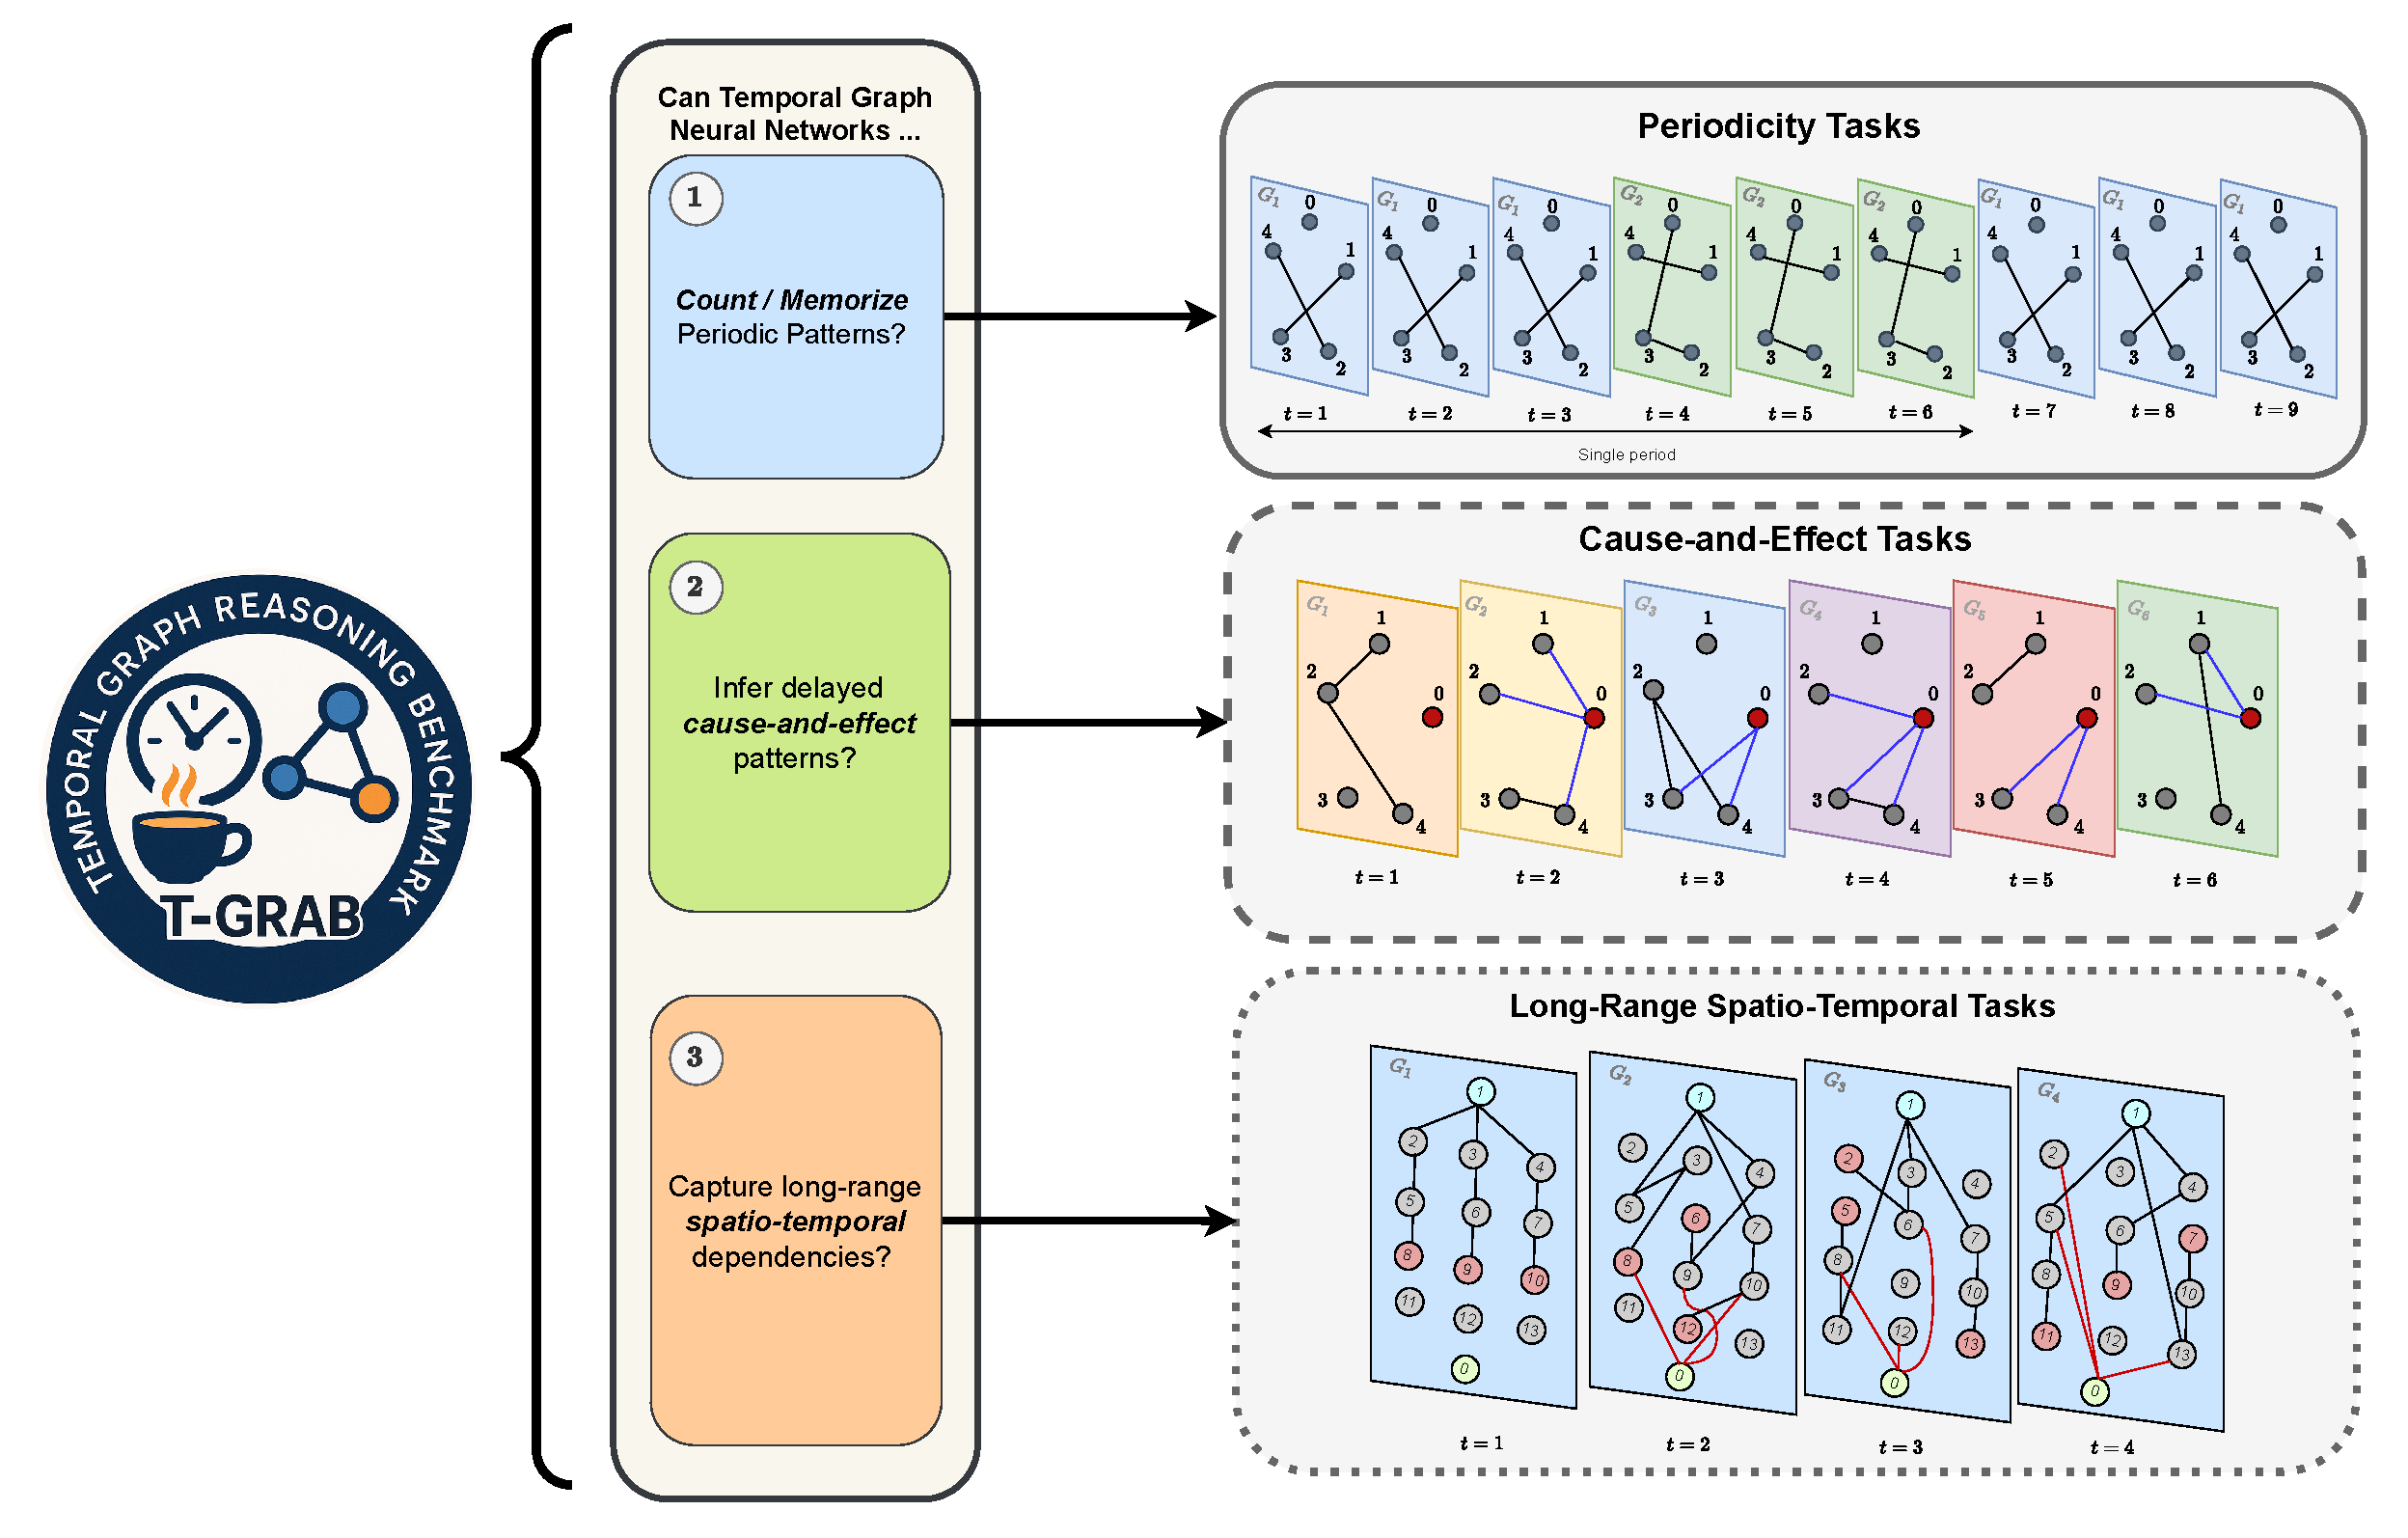
\includegraphics[width=\textwidth, keepaspectratio]{figs/T-GRAB Crown Jewel.drawio.pdf}
% \end{figure}


% \begin{figure}[H]
%     \centering
% %     \begin{minipage}{0.6\textwidth}
% %         \centering
%         \includegraphics[width=0.6\linewidth]{figs/TGRAB_flow.png}
% %     \end{minipage}
%     \caption{The workflow of T-GRAB } \label{fig:workflow}
% \end{figure} 



\section{Temporal Graph Preliminaries}
% We start by introducing some notations. 
% \paragraph{Notations}

% We first give a formal definition of discrete time dynamic graphs. 

\begin{definition}[Discrete Time Dynamic Graphs] 
A \emph{Discrete Time Dynamic Graph} $\mathcal{G}$ is a sequence of graph snapshots sampled at regularly-spaced time intervals~\cite{kazemi2020representation}:
$ \mathcal G = G_1,G_2,G_3,\cdots,G_T.$
Each $G_t = (V_t, E_t, \mat X_t)$ is the graph at snapshot $t=1,\cdots, T$, where ${V}_t$, ${E}_t$ are the set of nodes and edges in ${G}_t$, respectively, and $\mat X_t\in \mathbb R^{|V_t| \times d}$ is the matrix of node features at time $t$. %Lastly, all timestamps $1 \leq t \leq T$. 
\end{definition}
%\ah{we don't need to add it but technically there are edge features as well. We didn't use for our experiment.}

%Note that is relatively straightforward to evaluate continuous time methods on discrete time dynamic graphs, while the other way around is more tedious~\cite{huangutg}.

In this work, we focus on tasks designed for Discrete Time Dynamic Graphs~(DTDGs). As Continue Time Dynamic Graph~(CTDG) methods can be applied on DTDGs as well~\cite{huangutg}, we benchmark the performance of both types of methods for comprehensive evaluation.
In our tasks, the set of vertices is the same at all time steps, i.e., $V_1=V_2=\cdots =V_t = \cdots$. Node features are also constant through time and consists of one-hot encoding of the $N$ nodes~(i.e., $d=N$ and $\mat X_t = \mat I$ is the identity matrix for all $t$). While dynamic graphs sometimes have edge features, we do not use any in \benchmarkname. We follow the methodology outlined in~\cite{huangutg} to evaluate CTDG methods on discrete time graphs by translating all edges in each graph snapshot $G_t$ into a batch of edges $\{(u,v,t) \mid (u,v)\in E_t\}$. 


% \ah{add notations for temporal graph learning, how the graphs are formulated}
% \gr{what do we need to add for temporal graph learning?}

%\gr{Add discussion on continuous time graphs and how we train models.}

% \ah{maybe add discussion on random graph generators, the assumption we made for generating temporal graphs, i.e. the underlying distribution is modeled by a random graph generator and it can be change over time, we can cite the LAD paper + other change point detection paper for this assumption}

\section{Synthetic Benchmark of Temporal Graph Learning Methods}
\looseness-1 We now describe the three task types in \benchmarkname: \textit{Periodicity Pattern} tasks, \textit{Cause-and-Effect} tasks, and \emph{Long-Range Spatio-Temporal} tasks.
Table~\ref{tab:data} shows the dataset statistics for tasks in \benchmarkname. 


\begin{table*}[t]
\caption{\benchmarkname dataset statistics and characteristics. } \label{tab:data} 
  \resizebox{\linewidth}{!}{%
  \begin{tabular}{ l | l l l l l l}
  \toprule
  Dataset & \# Nodes & \# Edges
  & \# Timestamp & Counting & Memorizing & Spatial Understanding \\ 
  \midrule
  Periodicity &  xx - xx& xx - xx & xx - xx & \cmark & \cmark & \xmark\\ 
  Cause and Effect &  xx - xx & xx - xx & xx - xx & \xmark & \cmark & \cmark\\ 
  Long Range Spatio-Temporal &  xx - xx & xx - xx & xx - xx & \cmark & \xmark & \cmark\\ 
  \bottomrule
  \end{tabular}
  }
\end{table*}



\subsection{Periodicity Tasks}\label{synth-benchmark:periodicity}

We introduce a family of synthetic tasks designed to evaluate the ability of Temporal Graph Learning~(TGL) methods to learn periodic structure through time. Solving these tasks requires counting and memorization capabilities, under both deterministic and stochastic settings.

\begin{definition}[Periodicity Tasks]
Let $k, n \in \mathbb{N}$. The task families $\Pdet{k,n}$ and $\Psto{k,n}$ are defined based on a repeating pattern $p$ where each integer $i \in \{1,\dots,k\}$ appears $n$ consecutive times before cycling. At each time step $t$, let $i_t = (\lfloor t/n\rfloor \mod k) + 1$.

\ah{There is quite a bit of white space here, if needed, we can compress.}

In $\Pdet{k,n}$, the dynamic graph $\mathcal{G} = G_1, G_2, \dots$ is a periodic sequence alternating between $k$ fixed static graphs $G_1, \dots, G_k$, i.e., $G_t = G_{i_t}$.

In $\Psto{k,n}$, each $G_t$ is sampled from one of $k$ distributions $D_1, \dots, D_k$ over static graphs (e.g., Erd\H{o}s-Rényi~(ER)~\cite{erdos1960evolution}, Stochastic Block Model~(SBM)~\cite{holland1983stochastic}), with $G_t \sim D_{i_t}$. The resulting sequence is stochastic, but the distribution pattern follows the same periodic structure as in $\Pdet{k,n}$.
\end{definition}

\looseness-1 For example, a task in $\Pdet{k=3,n=2}$  will correspond to a dynamic graph $\mathcal G = G_1,G_1,G_2,G_2,G_3,G_3,G_1,G_1,\cdots\ $, where $G_1,G_2,G_3$ are static graphs. An illustration of another task in $\Pdet{k,n}$ is shown in Figure~\ref{fig:periodicity}.
\begin{figure}
    \centering
    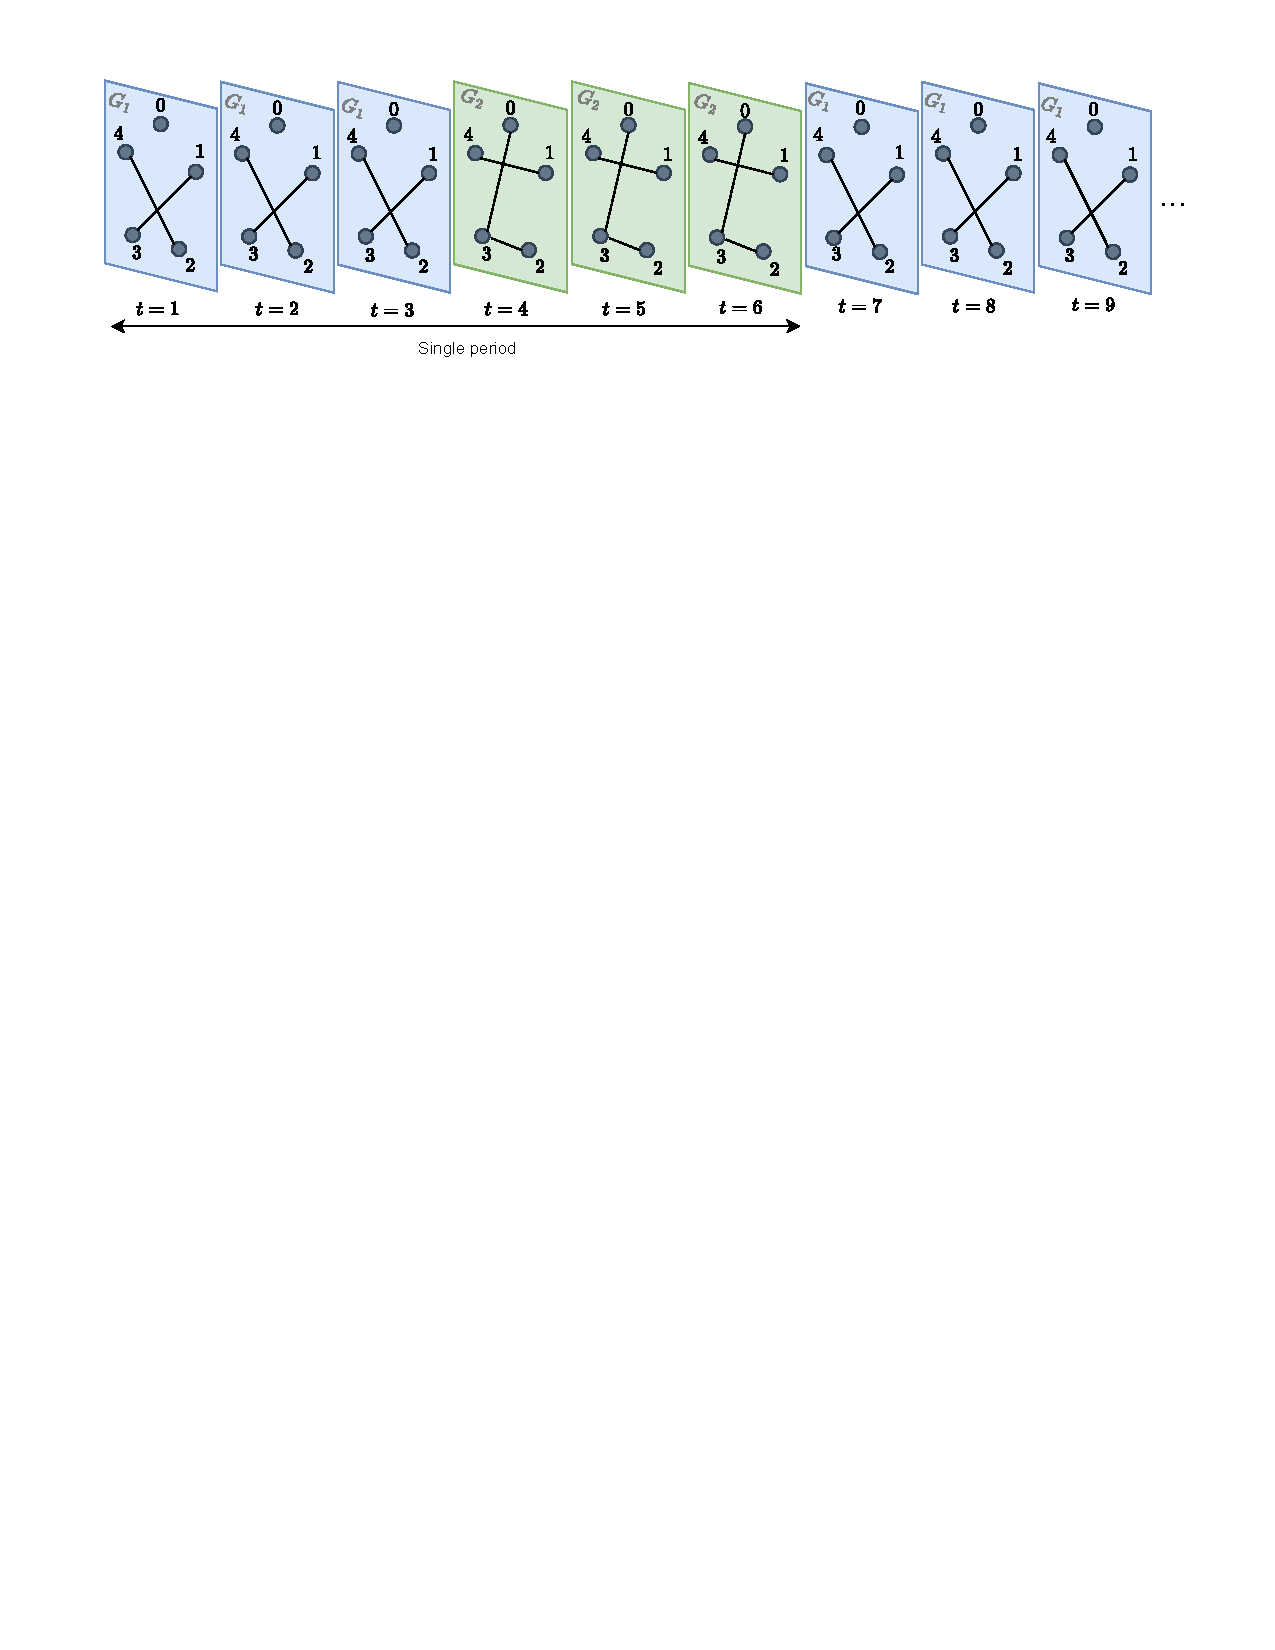
\includegraphics[width=\linewidth]{figs/periodicity/Fixed_ER/(2, 3)_dataset.pdf}
    \caption{A periodic task in $\Pdet{k=2,n=3}$ containing two unique snapshots, each repeated three times within a single period. }
    \label{fig:periodicity}
\end{figure}


\paragraph{Task objectives.}
Tasks in $\Pdet{k,n}$ test the counting and memory capacity of TGL methods. The parameter $k$ controls the length of the pattern and thus the memory demand, while $n$ governs how long each graph is repeated and tests the model's ability to count. For instance, solving a task in $\Pdet{2,n}$ requires counting up to $n$ before switching graphs, while solving a task in $\Pdet{k,1}$ requires memorizing $k$ static graphs. Tasks in $\Psto{k,n}$ introduce stochasticity, requiring models to reason over distributions rather than fixed structures, increasing the complexity while retaining the same periodic structure.



% \subsection{Periodicity Pattern Tasks}\label{synth-benchmark:periodicity}
% \looseness-1 We first introduce a set of tasks to investigate the ability of TGL methods to learn periodic patterns. The tasks we propose have diverse characteristics~(e.g., deterministic vs. probabilistic). To solve these tasks, TGL methods should be able to perform counting of some form and to memorize patterns or distributions. All the periodicity tasks we propose can be described using the following unified formal definition:

% \begin{definition}
% An instance of a \emph{periodic task} is defined by a tuple $(\mathcal{D},p)$, where $\mathcal{D} = \{D_1,\cdots, D_k\}$ is a set of $k$ distributions over static graphs, and $p$ is a \emph{pattern} of distributions~(i.e., a sequence of integers between $1$ and $k$)  to be repeated through time. If $p = (i_1,i_2\cdots,i_m)$, a dynamic graph $\mathcal{G} = G_1,G_2,G_3,\cdots$ drawn from the task $(\mathcal{D},p)$ will be such that each $G_t$ is drawn from the distribution $D_{i_t}$ where $i_t = (t \mod k)+1$.
% \end{definition}

% \looseness-1 To illustrate this definition, a dynamic graph $\mathcal G = G_1,G_2,G_3,\dots$ drawn from the periodic task $(\mathcal D = \{D_1,D_2\},p=(1,2))$ will be such that each $G_t$ is either independently drawn from $D_1$ (if $t$ is odd) or from $D_2$ (if $t$ is even). The distributions over static graphs mentioned in the definition can be any distribution from which~(static) graphs can be drawn, e.g., Erd\H{o}s-Renyi~(ER)~\cite{erdos1960evolution} or the Stochastic Block Model~(SBM)~\cite{holland1983stochastic}. In our experiments, we will always consider patterns $p$ of the form $1, 1, \dots, 2, 2, \dots, k, \dots, k$ where each number is repeated some fixed number of times.

% \paragraph{Deterministic periodic tasks}
% \looseness-1 We start by giving a very simple example of such a periodic task by letting each distribution $\mathcal{D}_k$ be a discrete distribution with all its probability mass concentrated on some static graph $G_k$. For example, let $G_1,G_2$ be two static graphs, and consider the deterministic distributions $D_1,D_2$ having all their mass on $G_1$ and $G_2$ respectively~(i.e., $\mathbb{P}_{G\sim D_1}[G=G_1] = 1$ and $\mathbb{P}_{G\sim D_2}[G=G_2] = 1$). Then, the periodic task $(\mathcal D =\{D_1,D_2\}, p = (1,2)))$ corresponds to a  dynamic graph alternating between two static graphs: $\mathcal G = G_1,G_2,G_1,G_2,G_1,G_2,\cdots$. We use $(\mathcal \{G_1,G_2\}, p = (1,2)))$ to denote such deterministic periodic tasks, directly specifying the graphs rather than the deterministic distributions. 

% This task can be made more difficult in two ways. First, we can increase the number of time each static graph is repeated, e.g., $(\{G_1,G_2\},  p = (1,1,1,2,2,2))$ will correspond to the dynamic graph $\mathcal G = G_1,G_1,G_1,G_2,G_2,G_2,G_1,G_1,G_1,\cdots\ .$ Alternatively, we can alternate between more than 2 graphs, e.g., $(\{G_1,G_2,G_3\}, p = (1,2,3))$ corresponds to the dynamic graph $\mathcal G = G_1,G_2,G_3,G_1,G_2,G_3,G_1,\cdots$.

% We denote the set of deterministic tasks alternating between $k$ static graphs each repeated $n$ times by $\Pdet{k,n}$. An example of a task in $\Pdet{k,n}$ is illustrated in Figure~\ref{fig:periodicity}.

% \begin{figure}[H]
%     \centering
%     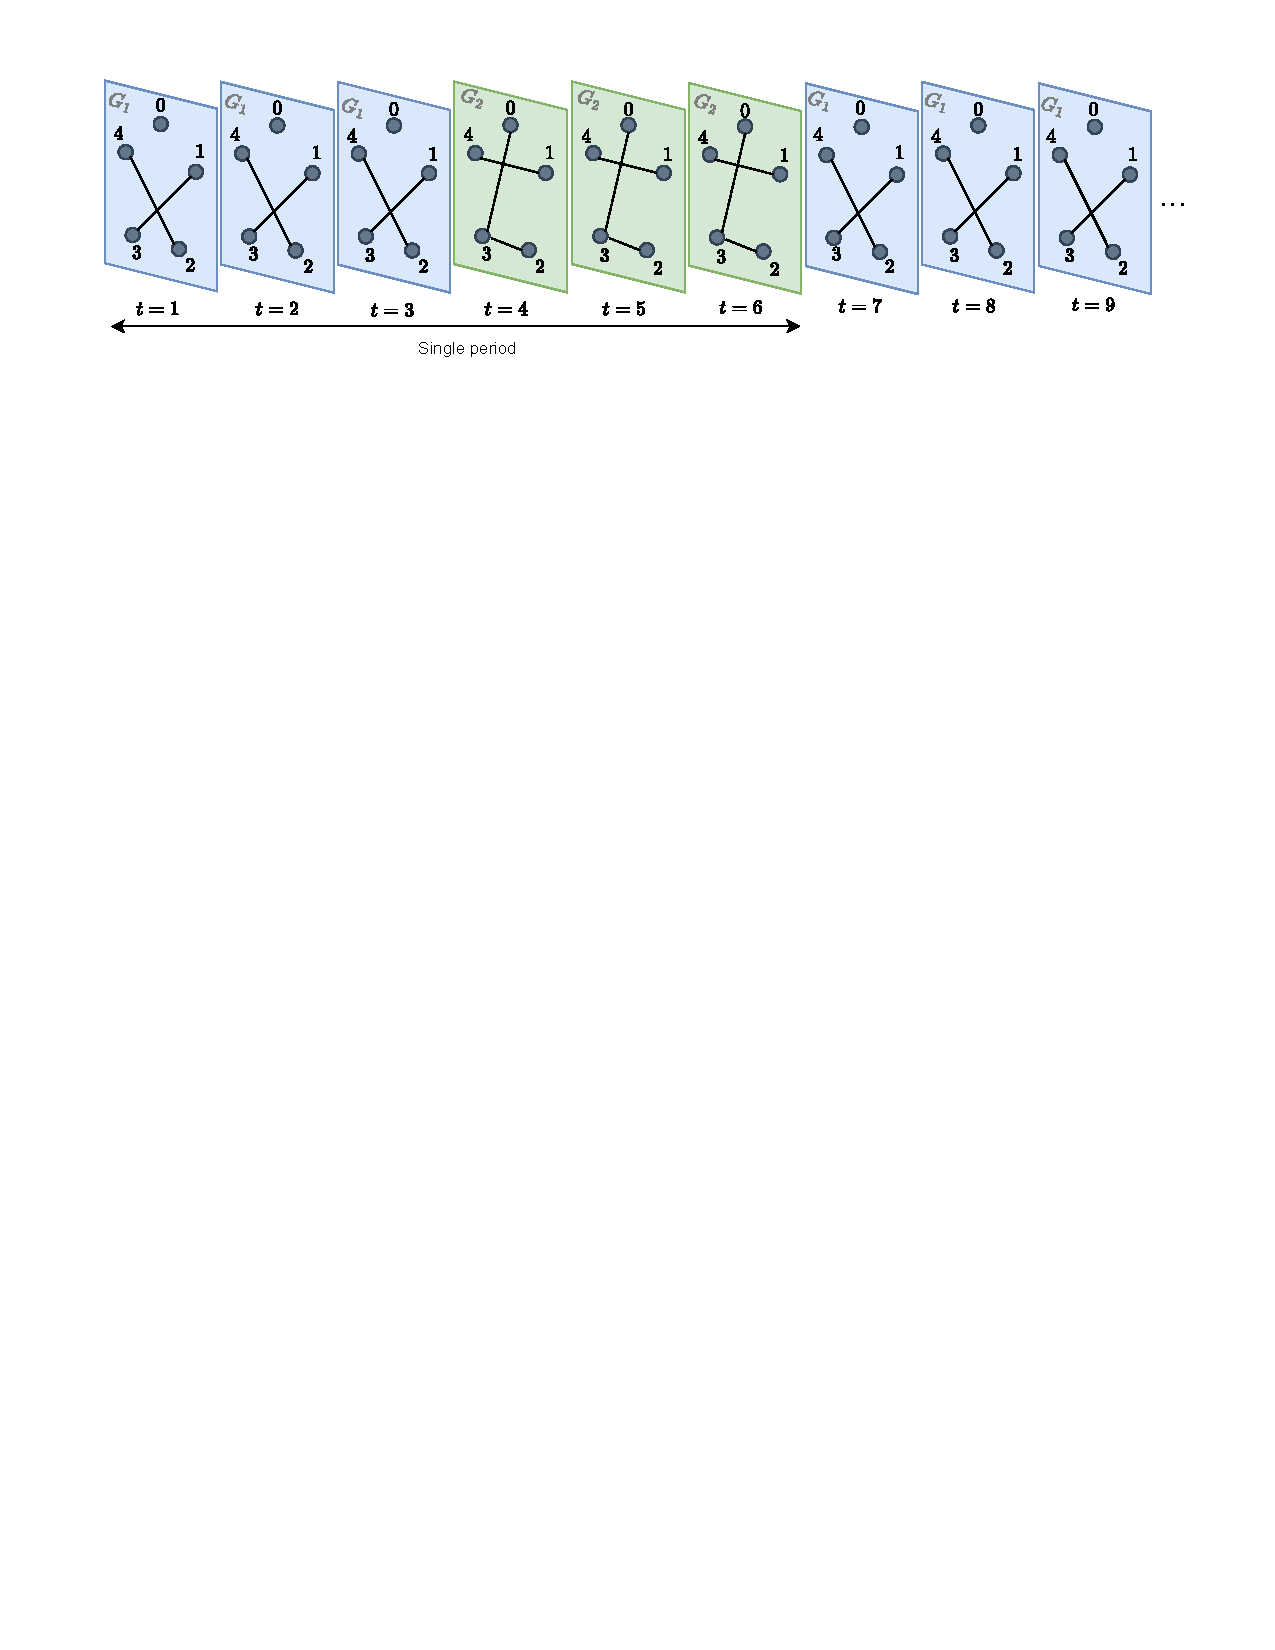
\includegraphics[width=\linewidth]{figs/periodicity/Fixed_ER/(2, 3)_dataset.pdf}
%     \caption{An illustration of a periodic task in $\Pdet{k=2,n=3}$ containing two unique snapshots, each repeated three times within a single period. }
%     \label{fig:periodicity}
% \end{figure}


% \paragraph{Stochastic periodic tasks}
% We will call a periodic task $(\mathcal D, p)$ stochastic if at least one distribution in the set $\mathcal D$ is not deterministic. Similarly to the deterministic case, we will use $\Psto{k,n}$ to denote the set of stochastic periodic tasks of the form $(\mathcal D = \{D_1,\cdots, D_k\},p=(1,1,\cdots,1,2,\cdots,2,\cdots,k,\cdots,k))$, where each integer in the pattern is repeated $n$ times. Natural choices for the distributions $D_i$ include Erd\H{o}s-Renyi~(ER)~\cite{erdos1960evolution} and the Stochastic Block Model~(SBM)~\cite{holland1983stochastic}. In our experiments we will consider tasks in $\Psto{k,n}$ where e.g. each $D_i$ is a SBM distribution with a different community structure.

% \paragraph{Task objectives}
% The set of tasks $\Pdet{k,n}$ is meant to test the counting and memory capacity of TGL methods.
% When $n=1$, the task is very similar to the copy task that has been used as a test bed to study neural sequence models~\cite{le2015simple,arjovsky2016unitary,tallec2018can}. As $k$ increases, the tasks gets harder w.r.t. the memory capacity since the model needs to remember longer sequences to repeat.
% The hyper-parameter $n$ allows one to test the counting ability of TGL models. Indeed, to succeed at a task in e.g. $\Pdet{2,n}$, the model needs to be able to count up to $n$ to know when to switch between the two graphs. 
% The two hyper-parameters $k$ and $n$ therefore control the difficulty of the periodicity task $\Pdet{k,n}$ on two different axes: $k$ is related to the memorization ability while $n$ is related to the counting ability of the models. 
% In a similar fashion, the set of tasks $\Psto{k,n}$ also test the counting and memory capacity of TGL methods, with the additional complexity that models now need to be able to reason with the uncertainty of stochastic latent structures instead of purely deterministic static graphs in the patterns. 
% % \item Another natural task to test the counting ability would be $(\{G_1,G_2\},\ttt{12}^n)$ for increasing values of $n$. $G_1$ and $G_2$ could be identical except for an additional motif appearing in $G_1$.

% %Lastly, it is worth mentioning that the set of tasks in $\Pdet{k,n}$  have the Markov property of order $kn-1$: knowledge of the last $kn-1$ graphs in the sequence is sufficient to exactly predict the  graph at the next time step. 

\subsection{Delayed Cause-and-Effect Tasks}
\looseness-1 To evaluate TGL methods' ability to learn delayed causal effects, we introduce the \emph{delayed cause-and-effect tasks}. In these tasks, we sample a sequence of graphs from a distribution (e.g., Erd\H{o}s-Rényi). A special node, called the memory node, is then added at each time step and connected to nodes involved in edges \(\lag\) time steps earlier. We formalize the task as follows:

\begin{definition}[Delayed Cause-and-Effect Task]
Let \(\lag \in \mathbb{N}\). The \emph{delayed cause-and-effect task} family \(\causeeffect{\lag}\) consists of dynamic graphs \(\mathcal{G} = G_1, G_2, \dots\) generated as follows: First, each graph \(G_t = (V, E_t)\) is sampled independently from a distribution \(D\) over static graphs, where \(V = \{v_1, \dots, v_n\}\) is the set of nodes, shared across time steps. For \(t > \lag\), the graph \(G_t\) is augmented by introducing a memory node \(v_{\mathcal M}\) and connecting it to the nodes involved in edges at time \(t - \lag\):
\[
V \leftarrow V \cup \{v_{\mathcal M}\}, \quad E_t \leftarrow E_t \cup \left\{ (v_{\mathcal M}, u), (v_{\mathcal M}, v) \mid (u,v) \in E_{t-\lag} \right\}  \text{ for } t > \lag.
\]
\end{definition}

\looseness-1 In other words, the model needs to remember nodes that were connected to each other at $E_{t-l}$ to predict the edges of the memory node at time $E_t$. An example of this task is illustrated in Figure~\ref{fig:memnode}. As \(\lag\) increases, the task becomes more challenging in terms of the memory capacity required from the model. Key factors that influence the difficulty of this task include the number of nodes and edges in the graphs \(G_t\), but in our experiments, we focus on varying \(\lag\) and denote this set of tasks by \(\causeeffect{\lag}\). Since only the edges involving the memory node can be predicted~(the other ones being completely random), only the accuracy of predicting the edges involving the memory node will be reported in our experiments.

 \begin{figure}
    \centering
    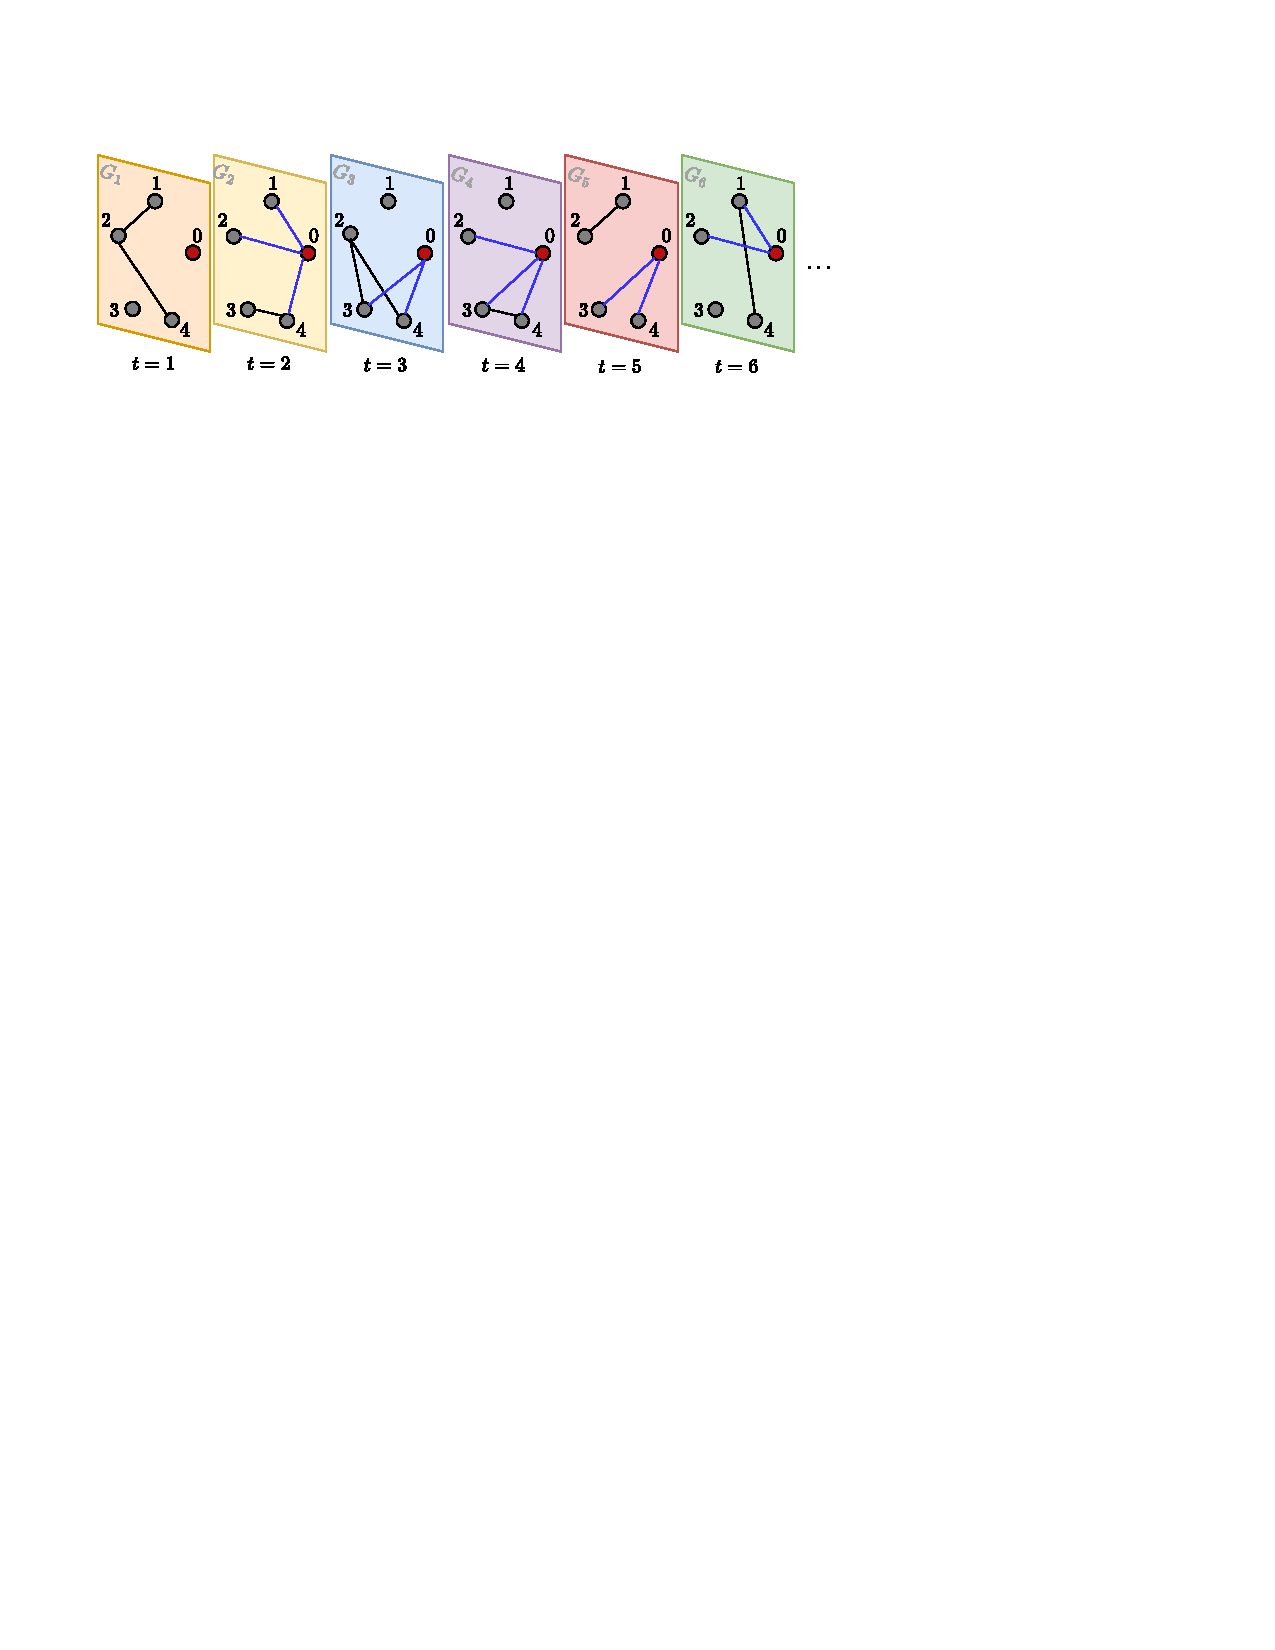
\includegraphics[width=0.8\linewidth]{figs/memory_node/lag=1.pdf}
    \caption{An illustration of a delayed cause and effect dataset with a lag $\lag=1$ of one timestep between cause and effect. The black and blue edges represent the cause and effect subgraphs, respectively. The cause subgraph consists of nodes indexed from $1$ to $n$. In the effect subgraph, the memory node~(node 0) connects to nodes from the cause subgraph at the previous timestep, provided their degree is at least one. }
    \label{fig:memnode}
\end{figure}

\paragraph{Task objectives}
In the delayed cause-and-effect tasks \(\causeeffect{\lag}\), TGNNs must not only propagate information over time (i.e., track which nodes were connected at time step \(t-\lag\)), but also identify the causal relationship that determines the memory node's connectivity. This requires models to recognize causal patterns through time. The difficulty of the task is controlled by the hyperparameter \(\lag\): as \(\lag\) increases, the model needs to retain information for longer periods, making it harder to identify the cause-and-effect relationships. In the following task, we introduce a spatial component to the pattern, allowing the difficulty to be controlled on two axes: time and space. 



% \subsection{Delayed Cause-and-Effect Tasks}
% \looseness-1 To test the abilities of TGNNs to learn delayed causal effects, we now present the  \emph{delayed cause-and-effect tasks}. In this task, we first sample a sequence of graphs randomly according to some distribution (e.g., Erdos-Renyi distribution). Next, we designate a special node called the memory node, that is only connected to nodes that were involved in an edge $\lag$ timesteps before. We formalize this task in the following definition: 

% \begin{definition}[Cause and effect task]
% An instance of the \emph{delayed cause and effect task} is specified by a tuple $(D,\lag)$ where $D$ is a distribution over static graph and $\lag$ is a  lag duration. A dynamic graph $\mathcal G = G_1,G_2,\dots$ for this task is generated by first sampling each 
% graph $G_t = (V,E_t)$ interdependently from $D$. Here we assume that the set of nodes $V=\{v_1,\cdots,v_n\}$ is the same for all time steps. Then, each graph $G_t$ is augmented by adding the memory node $v_{\mathcal M}$ to the set of vertices and connecting it to all the nodes involve in edges at time $t-\lag$:
% $$ V \leftarrow V\cup \{v_{\mathcal M}\},\ \ \ E_t \leftarrow E_t \cup \{ (v_{\mathcal M}, u), (v_{\mathcal M}, v) \mid (u,v) \in E_{t-\lag}\} \text{ for } t > \lag. $$
% \end{definition}

% An illustration of a dynamic graph for the delayed cause and effect task is given in Figure~\ref{fig:memnode}.
% As the lag $\ell$ increases, the task becomes more difficult w.r.t.  the memory ability of the model. 
% Other key hyper-parameters controlling the difficulty of this task are the number of nodes and edges appearing in the graphs $G_t$. We will focus on the effect of the lag $\lag$ in our experiments and denote this set of tasks by $\causeeffect{\lag}$. Since only the edges involving the memory node can be predicted~(the other ones being completely random), only the accuracy of predicting the edges involving the memory node will be reported in our experiments. 


%  \begin{figure}[H]
%     \centering
%     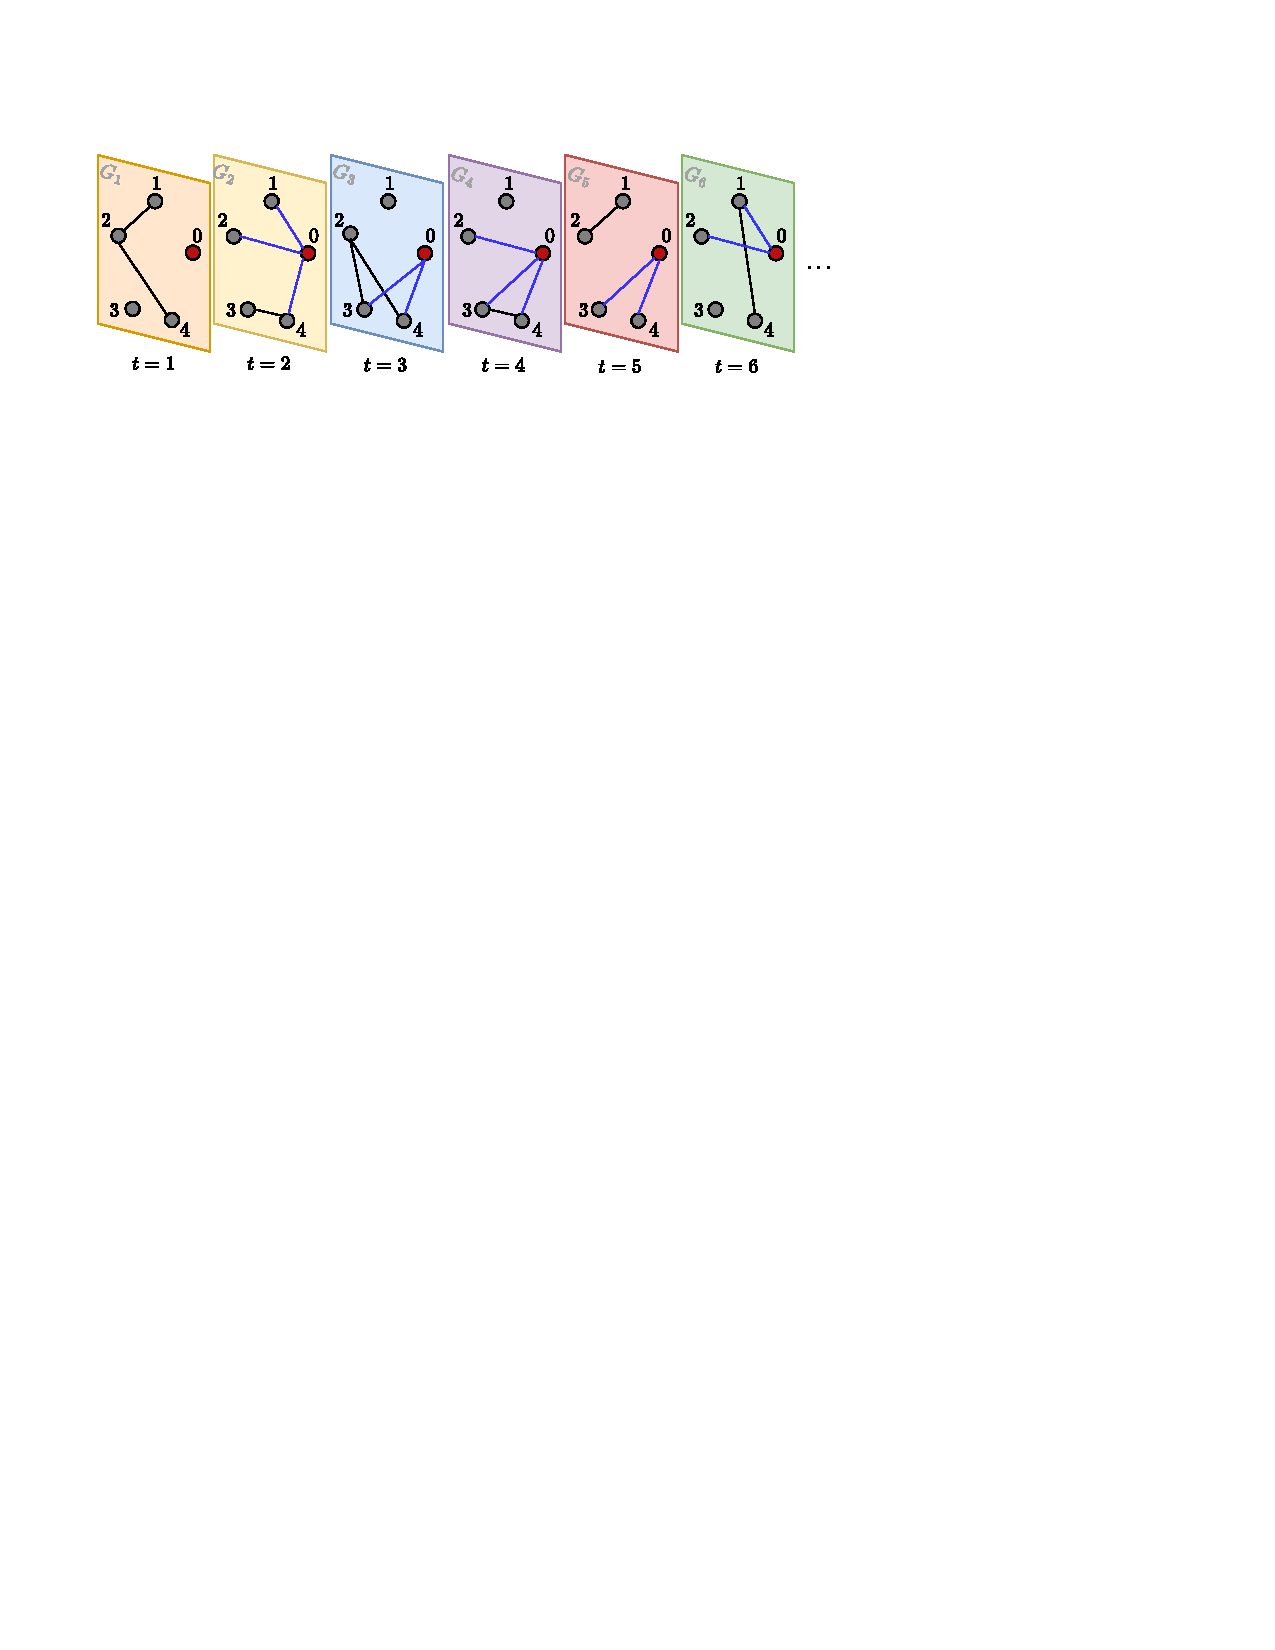
\includegraphics[width=0.8\linewidth]{figs/memory_node/lag=1.pdf}
%     \caption{An illustration of a delayed cause and effect dataset with a lag $\lag=1$ of one timestep between cause and effect. The black and blue edges represent the cause and effect subgraphs, respectively. The cause subgraph consists of nodes indexed from $1$ to $n$. In the effect subgraph, the memory node~(node 0) connects to nodes from the cause subgraph at the previous timestep, provided their degree is at least one. }
%     \label{fig:memnode}
% \end{figure}

% \paragraph{Task objectives}
% In delayed cause and effect tasks $\causeeffect{\lag}$, TGL methods not only need to propagate information through time~(which nodes where connected at time step $t-\lag)$), but also need to identify the causal pattern explaining the memory node's connectivity. Hence, the task requires TGL methods to identify causal patterns through time. The hyper-parameter $\lag$ controls the difficulty of the task: the higher it is, the longer the information needs to be retained and the more difficult it is to identify the cause and effect pattern. The following task we introduce will add a spatial component to the pattern, allowing the difficulty to be controlled on two axes: time and space. 


\subsection{Long-Range Spatio-Temporal Task}
Finally, to evaluate the ability of TGL methods to reason over both temporal and spatial dependencies, we introduce  \emph{long-range spatio-temporal tasks}. These tasks combine time delays with structural patterns, extending the delayed cause-and-effect setup to include long spatial paths.  At each time step, the graph contains paths originating from a source node \(v_{\mathcal S}\), while the target node \(v_{\mathcal T}\) connects to the endpoints of the paths generated $\lag$ time steps before.
 The task is formalized as follows:


\begin{definition}[Long-Range Spatio-Temporal Task]
\looseness-1 Let \(\lag, d, P \in \mathbb{N}\). The \emph{long-range spatio-temporal task} family \(\longrange{\lag,d,P}\) is defined over dynamic graphs \(\mathcal{G} = G_1, G_2, \dots\), where each snapshot $G_t = (V, E_t)$ has a fixed node set $V = \{v_{\mathcal S}, v_{\mathcal T}, v_1, \dots, v_{N}\}$. The edge set $E_t$ consists of $P$ disjoint paths of length $d$ from the source node $v_{\mathcal S}$ through randomly chosen intermediate nodes. For $t > \lag$, $E_t$ additionally includes $P$ edges from the target node $v_{\mathcal T}$ to the endpoints of the $P$ paths in $G_{t - \lag}$. Formally, for $t > \lag$:
$
E_t = \bigcup_{p=1}^P \{(v_{\mathcal S}, u_1^{(t,p)}), (u_1^{(t,p)}, u_2^{(t,p)}),\dots, (u_{d-1}^{(t,p)}, u_d^{(t,p)})\} \cup \{(v_{\mathcal T}, u_d^{(t-\lag,p)})\}$, where the nodes $u^{(t,p)}_{i}$ for $i=1,\dots,d$, $p=1,\dots,P$ are drawn at random in $\{v_1,\dots,v_N\}$~(without replacement).
\end{definition}\label{def:long_range}


Intuitively, we can treat node $v_\mathcal{S}$ as the \textit{progenitor} of some signal that 1) reaches a set of nodes that are spatially separated from $v_\mathcal{S}$ by a distance $d$ and 2) whose effect (connecting the nodes that it reached to node $v_\mathcal{T})$ is additionally delayed by $l$ timesteps.
An illustration of a dynamic graph for the Long-Range Spatio-Temporal task is given in Figure~\ref{fig:longrange}. Here, given $P = 3, d = 3$, observe that at $t = 1$, $S$ is connected to 3 paths of length 3. The terminal nodes of these paths, namely $8, 9, 11$ are then connected to target $T$ after a lag of 1. We will focus on the effect of the lag $\lag$  and distance $d$ in our experiments and set the number of path $P$ to $3$ in all tasks, which we will denote by $\longrange{\lag,d}$.

\begin{figure}
    \centering
    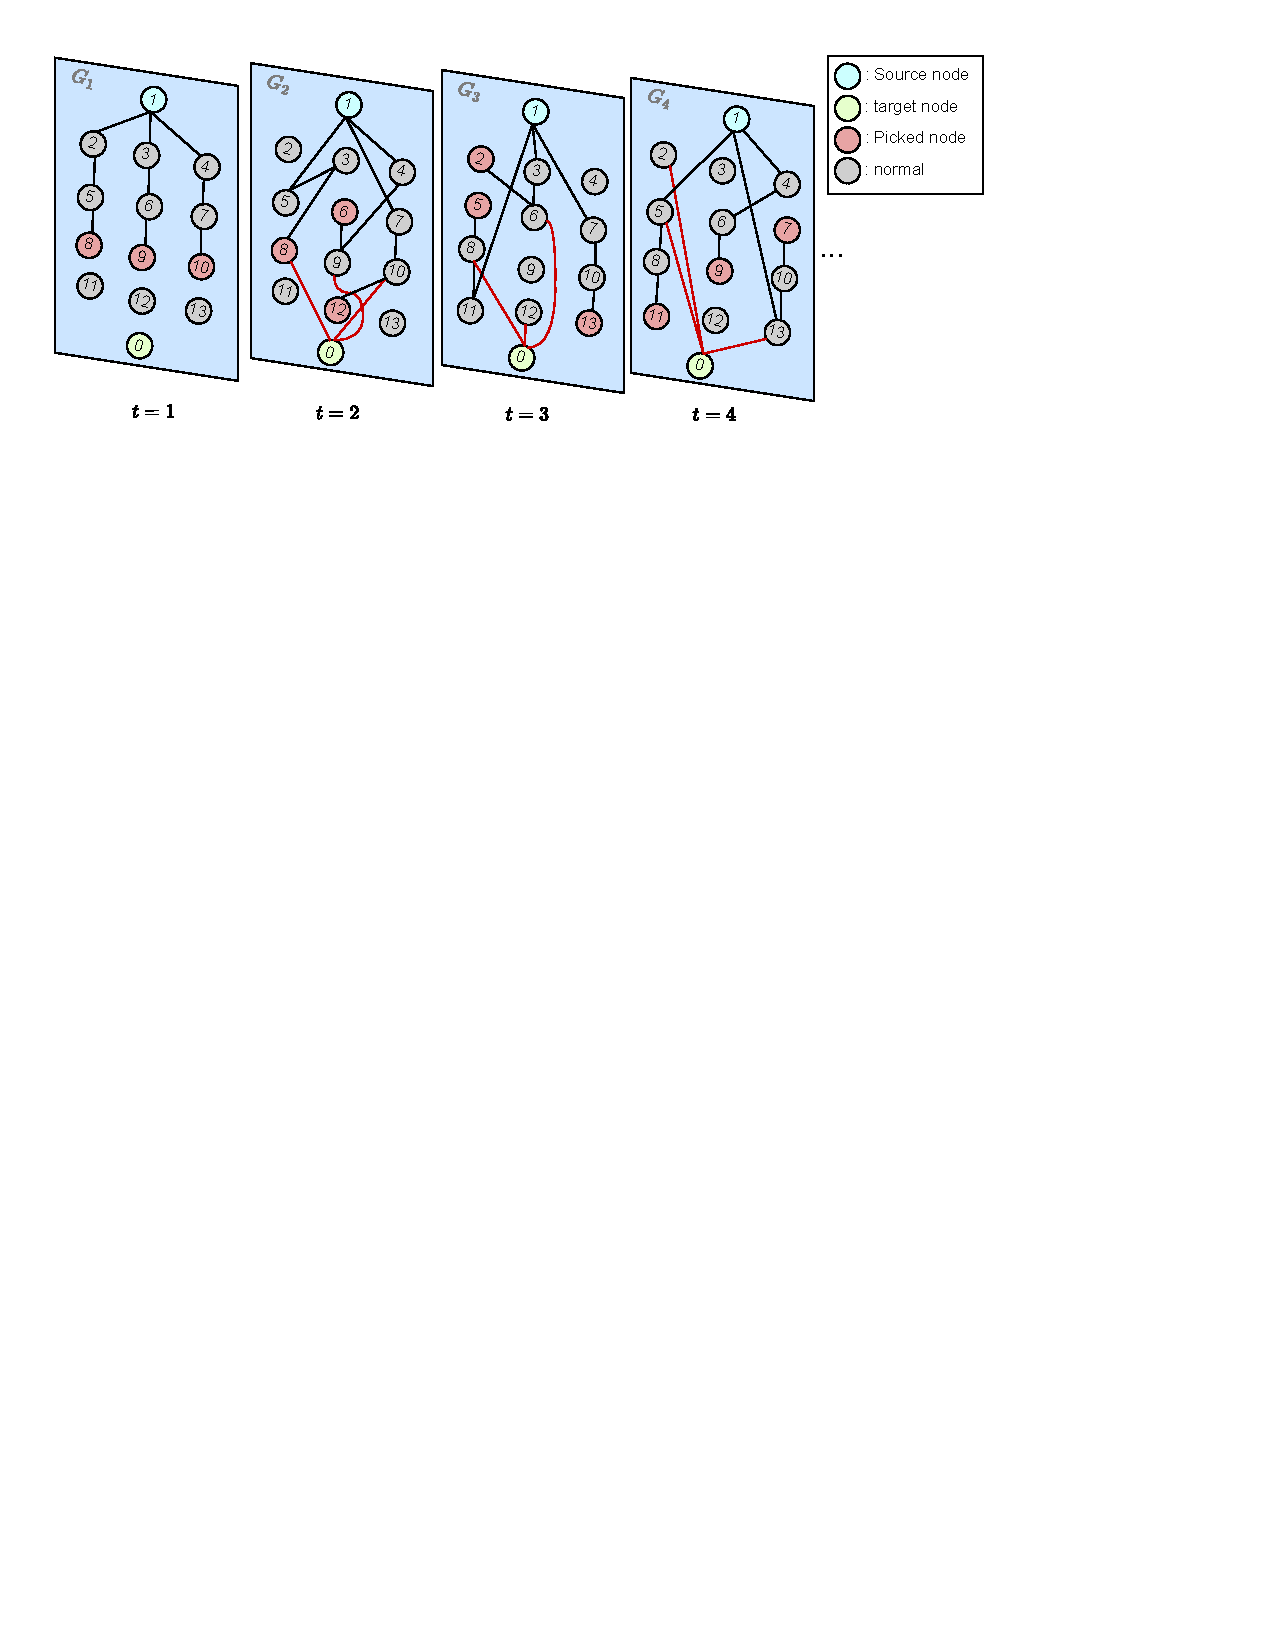
\includegraphics[width=0.8\linewidth]{figs/long_range/fig.pdf}
    \caption{An illustration of a long-range dependency task with parameters   $\ell=1$, $d=3$ and $P=3$ is shown. In our datasets, the nodes indexed as $1$ and $0$ are designated as the \textit{source} ($S$) and \textit{target} ($T$) nodes, respectively. The \textit{picked} nodes represent the endpoints of the $P$ paths, each of which connects to $T$ after $\ell$ time steps.}
    \label{fig:longrange}
\end{figure}

\paragraph{Task objectives}
\looseness-1 In dynamic graphs, there are two natural notions of distances: distance between time steps and distance between nodes~(e.g., shortest path). Robust and powerful TGL methods should thus be able to reason and identify patterns simultaneously across these two dimensions. Tasks in \(\longrange{\lag,d}\) challenge TGL methods to jointly reason over long-term temporal dependencies and multi-hop spatial paths. The lag \(\lag\) determines how long information must be retained, while the distance \(d\) controls how far it must be propagated through the graph structure. This dual complexity makes the task a powerful benchmark for assessing the depth of spatio-temporal reasoning in TGL models.

\section{Experiments}\label{sec:experiments}
We compare a range of TGL methods on \benchmarkname's tasks~(complete experimental details can be found in \Cref{appendix:experimental-details}): four continuous-time~(CTDG) methods~(DyGFormer~\cite{dygformer}, CTAN~\cite{ctan}, TGN~\cite{tgn} and TGAT~\cite{tgat}), three discrete-time~(DTDG) methods~(EvolveGCN~\cite{evolvegcn}, T-GCN~\cite{tgcn}, and GC-LSTM~\cite{gclstm}), two static graph methods~(GCN~\citep{gcn} and GAT~\cite{gat}), and two baselines~(\textit{persistence}, which always predicts the edges present at the previous time step, and $\text{Edgebank}_{\infty}$\citep{poursafaei2022betterevaluationdynamiclink}).

\ah{we need to add some details of how we apply CTDG methods on DTDG datasets. We can discuss here if we have space or put it in experiment details.}

\paragraph{Evaluation}
% Since the dynamic graphs we consider are relatively small, we do not have to rely on negative sampling for our evaluation, which has many drawbacks~\cite{poursafaei2022betterevaluationdynamiclink}, and instead evaluate the models by reporting the average $F_1$ score over all possible edges across all time steps in the test set.  For the periodicity tasks, all edges in the test set are included in the $F_1$ computation. For the  cause and effect and long range tasks, not all edges are included in the $F_1$ computation since only the edges involving the memory node can be predicted. Indeed, all the other edges are generated completely at random. Hence, for these tasks the $F_1$ is averaged only over the edges of the test set involving the memory node. 
Since the dynamic graphs in \benchmarkname are relatively small, we avoid the drawbacks of negative sampling~\cite{poursafaei2022betterevaluationdynamiclink} and instead evaluate models using the average $F_1$ score over all possible edges at each test time step. For periodicity tasks, all test edges are included in the $F_1$ calculation. In contrast, for the cause-and-effect and long-range tasks, only edges involving the memory/target node are considered, as all other edges are randomly generated and thus unpredictable. 

% \gr{TODO: 
% \begin{itemize}
%     \item we need to explain the proportion of train/valid/test in each subsection for each task
%     \item we need to explain how we trained the methods~(learning rates, batch sizes, basic TGL training loop, etc.). Most of it can go in the appendix but should pointed to here and a short summary given
% \end{itemize}
% }

% To identify the links of interest, we define a task-specific mask function $M^{\text{task}}_t: V_t \times V_t \rightarrow \{0, 1\}$, which selects a subset of node pairs $E^M_t = \{(u, v) \mid u, v \in V_t, M^{\text{task}}_t(u, v) = 1\}$. The $F_1$ score is then computed between the model's predictions and the ground truth for $E^M_t$ at each time step, and the results are averaged over all time steps.

% For periodicity tasks, the mask function $M^{\text{periodicity}}_t$ includes all possible node pairs in the graph, i.e., $\forall u, v \in V_t, M^{\text{periodicity}}_t(u, v) = 1$. In the memory-node task, the objective is to assess the model's ability to capture the causal subgraph centered around node zero, defined as:
% \[
% M^{\text{memnode}}_t(u, v) = 
% \begin{cases}
% 1, & \text{if } u.v = 0 \\
% 0, & \text{otherwise}
% \end{cases}
% \]
% A similar mask function is also applied for the spatial long-range dependency task.

\subsection{Periodicity Tasks}
\looseness-1 Recall from \Cref{synth-benchmark:periodicity} that the periodicity tasks are parameterized by $k$ and $n$. To evaluate the \textit{counting} abilities of TGNNs, we can fix $k = 2$ and vary $n$. To be successful in this setting, a given model needs to be able to 1) recognise whether a $G_i$ is equal to $G_1$ or $G_2$ (or whether or not it is sampled from $D_1$ or $D_2$ in the stochastic setting) and 2) keep a running count of these events to predict what comes next in the periodic sequence. We refer to the set of experiments under this setting as \textbf{counting periodicity experiments}: $\Pdet{2, n}$ and $\Psto{2, n}$, with $n \in \{ 1, 2, 4, 8, 16, 32, 64, 128 \}$. As $n$ increases, we can see that the task increases in difficulty as models are required to count longer sequences. 

\looseness-1 To probe the \textit{memorization} capabilities of TGNNs, we can conversely vary $k$ and fix $n = 1$. In this setting, a given model needs to be able to 1) determine which of $G_1 \dots G_k$ is some $G_i$ equal to (or which of $D_1 \dots D_k$ it is sampled from in the stochastic case) and 2) \textit{memorize} events in the past to determine what comes next in $k$-length periodic sequence. We refer to the set of experiments under this setting as \textbf{memorizing periodicity experiments}: $\Pdet{k, 1}$ and $\Psto{k, 1}$, with $k \in \{ 2, 4, 8, 16, 32, 64, 128, 256 \}$. As $k$ increases, the task increases in difficulty as it requires the model to memorize a longer sequence of past events. 

% Note that we did not include $k = 1$ as it is a degenerate case with only one graph type in the deterministic case or one distribution in the stochastic case. 

\textbf{Dataset Construction.} To construct the dynamic graph $\mathcal{G}$ for a deterministic counting/memorizing periodic task $\Pdet{k, n}$, we first sample $G_i$ for $i \in \{ 1, \dots k \}$ exactly once from an Erdős-Rényi model \citep{erdos1960evolution} $G^{(ER)}(n^{(\text{er})}, p^{(\text{er})})$, where we set $n^{(er)} = 100$ and $p^{(er)} = 0.01$ in our experiments. After obtaining $G_1, \dots, G_k$, we repeat each $G_i$ $n$ times as per the definition in \Cref{synth-benchmark:periodicity} to obtain $\mathcal{G}$.

On the other hand, given a stochastic task $\Psto{k, n}$, we \ad{Insert details here}.

Dataset statistics for counting periodicity and memorizing periodicity datasets under both deterministic and stochastic cases can be found in \Cref{appendix:periodicity-deterministic-stats}.

% \textbf{Counting Periodicity Experiments Results.} 
\textbf{Counting Periodicity Experiments Results.}  \ah{[Suggested section title.]\textbf{Can TGNNs count?}}
\Cref{fig:det_periodic_overall} presents our experimental results for both the \textit{counting periodicity experiments}. Here, we provide the $F_1$ scores averaged at all timesteps and additionally average $F_1$ scores at points where the sequence switches to a new pattern, i.e., at $t \in \{ n, 2n, 3n, \cdots \}$. We call the latter \textit{change-point evaluation} and should better indicate the ability of models to correctly \textit{count}, as opposed to evaluating the $F_1$ scores at all timesteps. 

\at{@Alireza, I've copied your analysis above. I think we should emphasize that the (All) evaluation sort of `lies', as if we look at the change-point evaluation, all models perform worse as $n$ increases.}

From \Cref{fig:det_periodic_overall}, we can see that among the CTDG models, TGAT performs well for smaller $n$, while DyGFormer emerges as a more consistent performer as $n$ increases. In the DTDG category, TGCN and GCLSTM generally achieve stronger results. Interestingly, both EvolveGCN-O and EvolveGCN-H perform worse than the static graph learning methods, GCN and GAT, which do not incorporate any temporal information. As expected, EdgeBank maintains constant performance across all $n$ values, as it always outputs the union of the two patterns, making its results independent of the period length. Additionally, the Persistence baseline improves with larger $n$, since it merely repeats the previous timestep’s snapshot, a simple strategy that proves highly effective at larger $n$ (e.g., 16, 32, 64, 128), even outperforming state-of-the-art models and revealing the challenges these models face in accurately counting and capturing pattern transitions over extended periods.

% Specifically, we define the counting task using $\Pdet{2, n}$, where within each period, a single graph is repeated $N$ times before switching to another graph, which is then also repeated $N$ times, as illustrated in Figure~\ref{fig:periodicity}. We refer to these as \textit{intra-repetitive periodicity} experiments. Furthermore, we analyze the models’ counting abilities by reporting their performance at each timestep, offering a detailed view of how effectively models track periodic patterns over time.
% \\
% In contrast, to assess memorization capabilities, we introduce experiments where multiple distinct patterns appear within a period without repetition, formally expressed as $\Pdet{k, 1}$ and $\Psto{k, 1}$. We refer to these as \textit{multi-pattern periodicity} experiments. The inclusion of probabilistic setups allows us to generalize the insights gained from deterministic tasks. 

% \subsubsection{Deterministic periodicity}
% In this section, we present an analysis of the models’ behavior on periodic tasks under deterministic conditions. To construct a $\Pdet{k, n}$ task in a deterministic setting, we generate the sequence $\mathcal{G}$ by sampling each graph $G_i$ (for all $i \in \{1, ..., k\}$) exactly once from an Erdős-Rényi model \citep{erdos1960evolution}, denoted as $G^{(ER)}(n^{(\text{er})}, p^{(\text{er})})$, where $n^{(\text{er})}$ and $p^{(\text{er})}$ correspond to the number of nodes and the probability of forming an edge between each pair of nodes, respectively. Throughout our experiments, we set $n^{(\text{er})} = 100$ and $p^{(\text{er})} = 0.01$. Table ~\ref{tab:det_periodic_datasets} summarizes the details of the synthetic datasets generated for two deterministic scenarios: \textit{intra-repetitive} and \textit{multi-pattern} periodic tasks.





\paragraph{Intra-repetitive periodicity $\Pdet{2, n}$.} As shown by Figure~\ref{fig:det_periodic_overall}, the performance of CTDG, DTDG, and baseline models on the $\Pdet{2, n}$ setting by averaging results over both the "all" timesteps and the specific "change point" timesteps. Here, \textit{change points} refer to the moments $t = \left\{0, n, 2n, 3n, ..., T\right\}$ when the graph snapshot switches to a new pattern. Focusing on these points helps evaluate the models' ability to correctly count, as we expect them to perform optimally at each transition, while still maintaining accurate repetition within each period. \\
To adjust the difficulty of the counting task, we progressively increase the value of $n$ and examine whether models can sustain high performance at both the change points and throughout the entire evaluation sequence. \\
Figure~\ref{fig:det_periodic_overall} summarizes the overall performance of CTDG, DTDG, and baseline models across different $n$ values. Among the CTDG models, TGAT performs well for smaller $n$, while DyGFormer emerges as a more consistent performer as $n$ increases. In the DTDG category, TGCN and GCLSTM generally achieve stronger results. Interestingly, both EvolveGCN-O and EvolveGCN-H perform worse than the static graph learning methods, GCN and GAT, which do not incorporate any temporal information. As expected, EdgeBank maintains constant performance across all $n$ values, as it always outputs the union of the two patterns, making its results independent of the period length. Additionally, the Persistence baseline improves with larger $n$, since it merely repeats the previous timestep’s snapshot, a simple strategy that proves highly effective at larger $n$ (e.g., 16, 32, 64, 128), even outperforming state-of-the-art models and revealing the challenges these models face in accurately counting and capturing pattern transitions over extended periods.\\
Finally, Figure~\ref{fig:(2,N)_per_timestep} offers a detailed, timestep-level view of model performance throughout the evaluation period. It shows that most models tend to lose accuracy at the start of each repetition phase and struggle to transition cleanly to the next pattern at the predefined change points (indicated by vertical lines). A notable observation is the sharp increase in performanceimmediately after these change points among dynamic graph learning methods, indicating that these models rely on seeing the new snapshot once before correctly adapting their predictions. 

\begin{figure}[t]
    % CTDG (2, n) all, (2, n) change points, (k, 1) all
    \centering
    \begin{subfigure}[b]{0.3\textwidth}
        \centering
        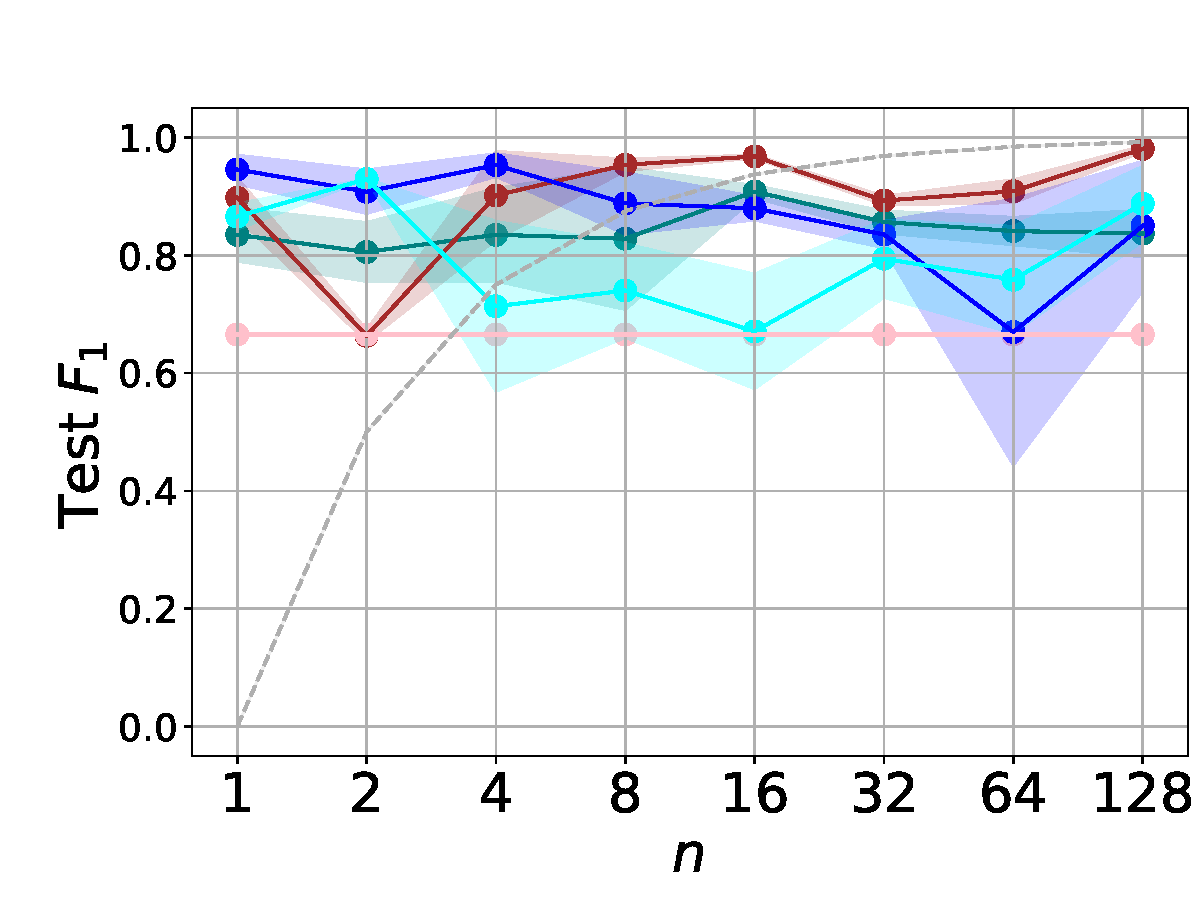
\includegraphics[width=\linewidth]{figs/periodicity/Fixed_ER/(2, n)CTDG_Test $F_1$.pdf}
        \caption{CTDG - $\Pdet{2,n}$ - All.}
        \label{fig:sub_ctdg_(2,n)_allstep}
    \end{subfigure}
    \begin{subfigure}[b]{0.3\textwidth}
        \centering
        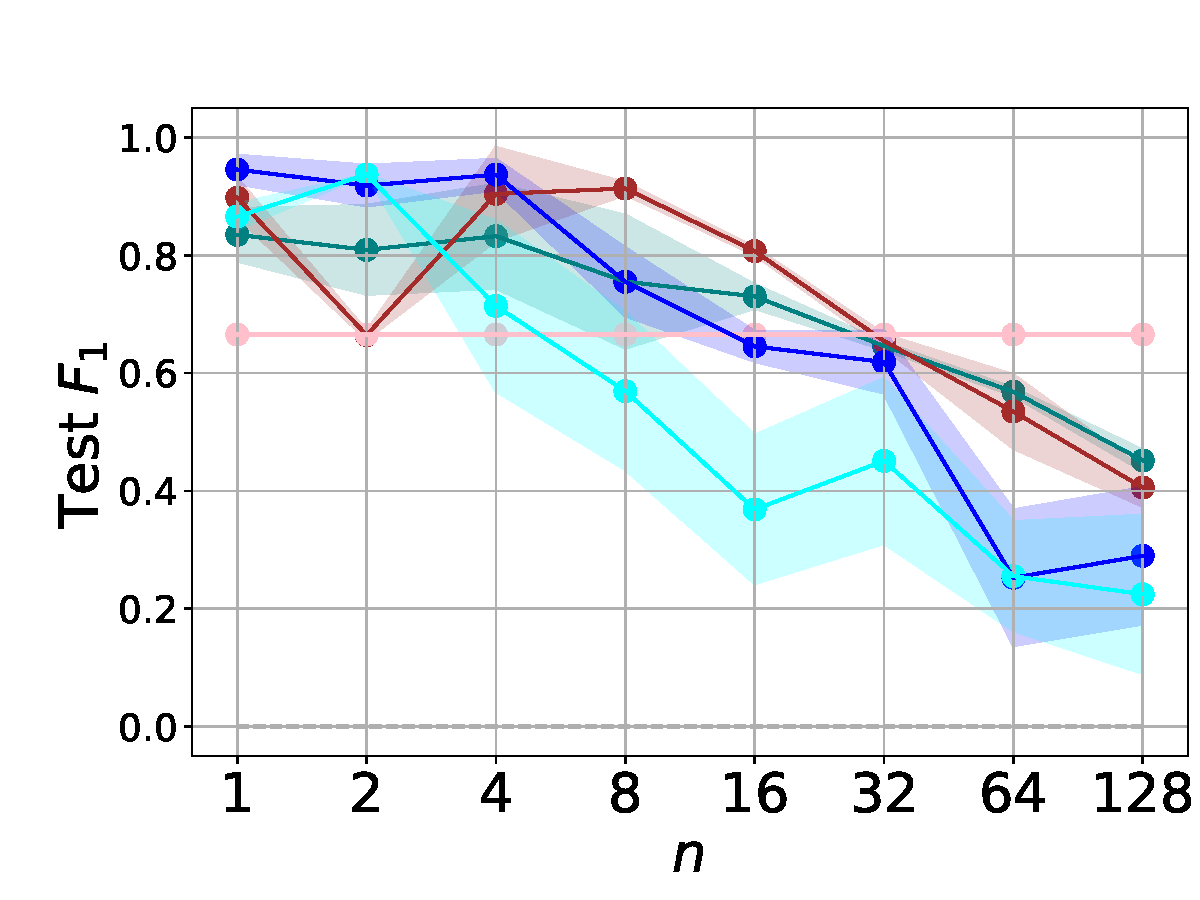
\includegraphics[width=\linewidth]{figs/periodicity/Fixed_ER/change_point/(2, n)CTDG_CP_Test $F_1$.pdf}
        \caption{CTDG - $\Pdet{2,n}$ - Change.}
        \label{fig:ctdg_(2,n)_changepoints}
    \end{subfigure}
        \centering
    \begin{subfigure}[b]{0.3\textwidth}
        \centering
        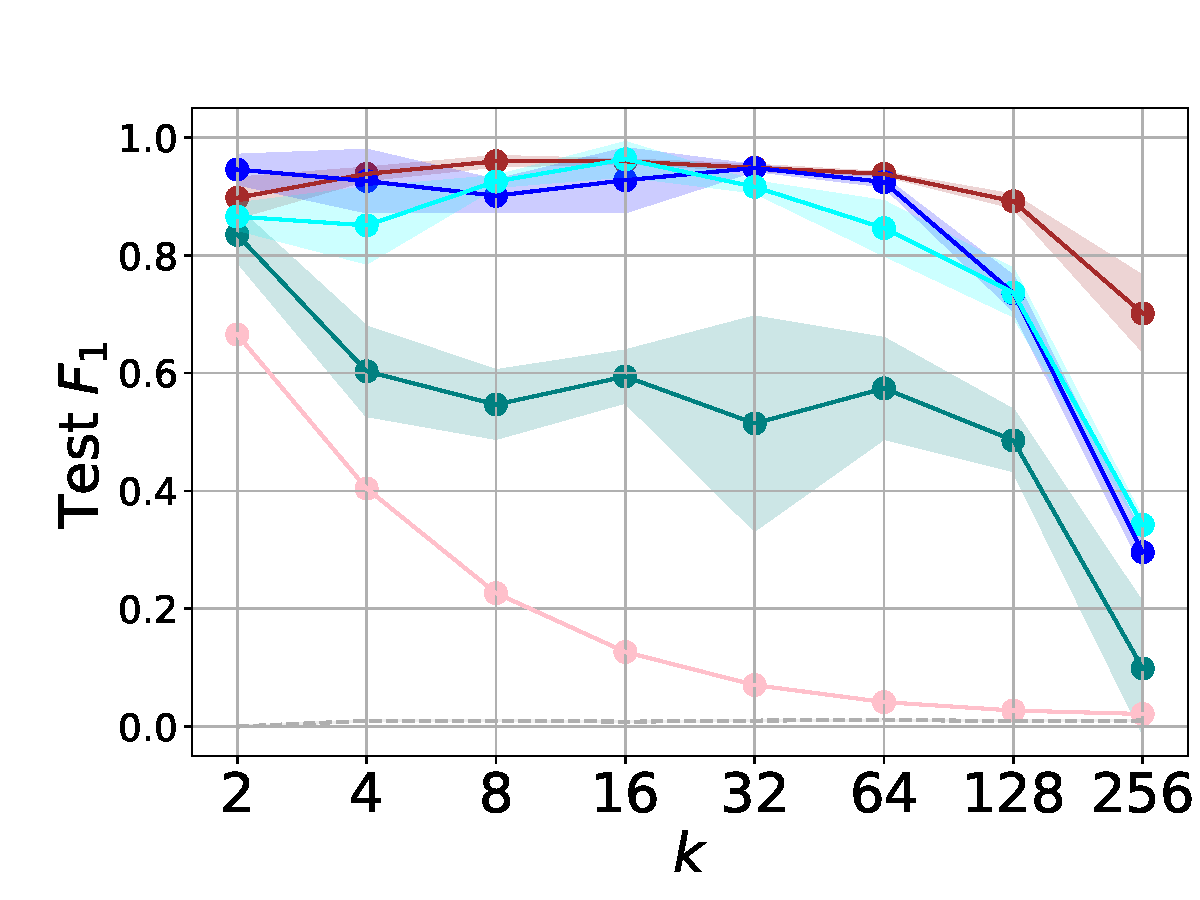
\includegraphics[width=\linewidth]{figs/periodicity/Fixed_ER/(k, 1)CTDG_Test $F_1$.pdf}
        \caption{CTDG - $\Pdet{k, 1}$ - All.}
        \label{fig:ctdg_(k, 1)}
    \end{subfigure}
    \begin{subfigure}[b]{0.08\textwidth}
        \centering
        \raisebox{14mm}{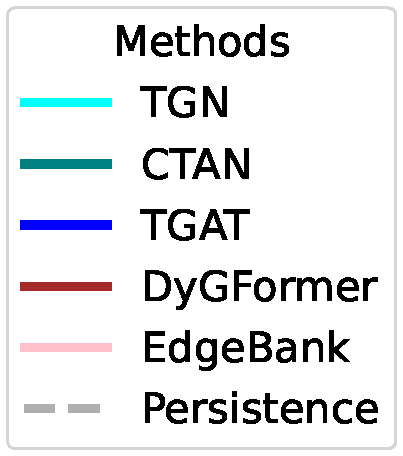
\includegraphics[width=\linewidth]{figs/legends/CTDG w persistence.pdf}}
    \end{subfigure}

    % DTDG (2, n) all, (2, n) change points, (k, 1) all
    \centering
    \begin{subfigure}[b]{0.3\textwidth}
        \centering
        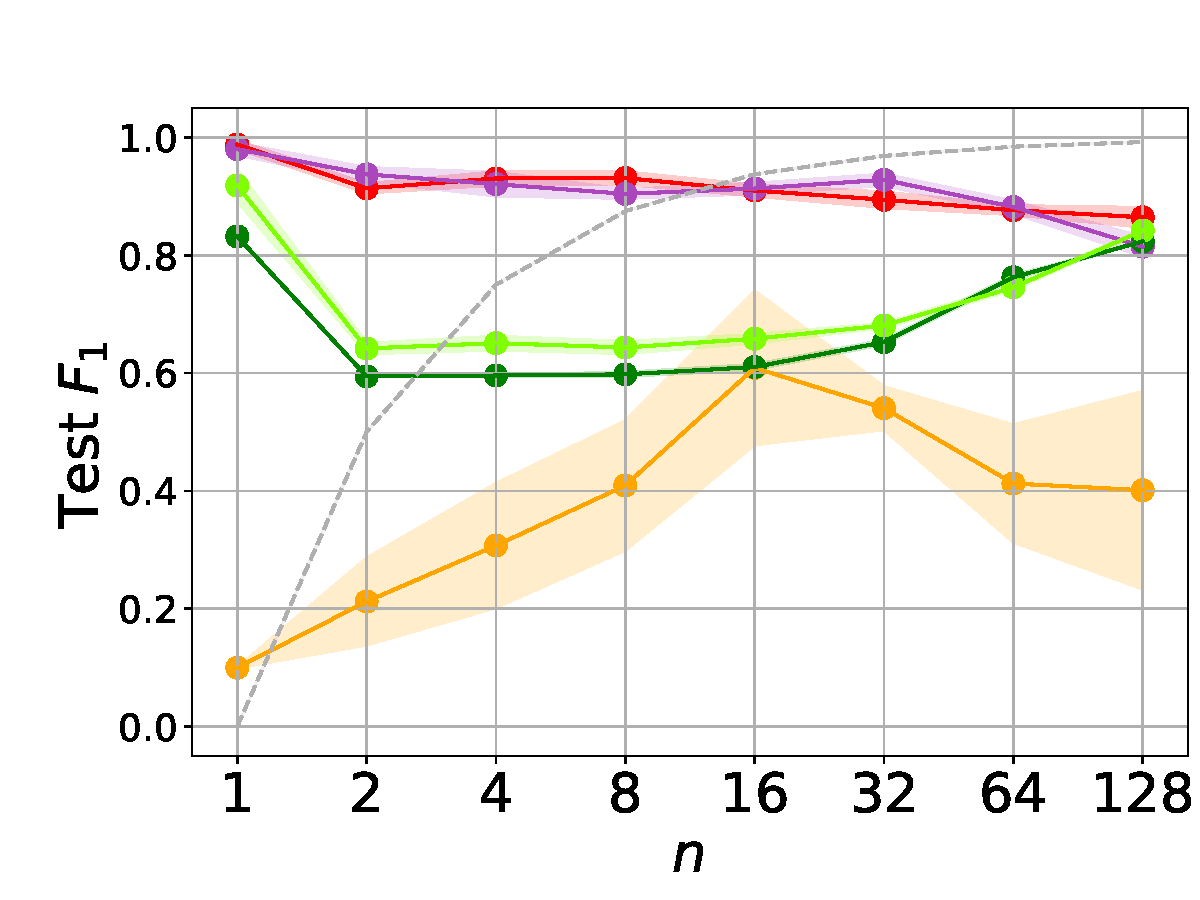
\includegraphics[width=\linewidth]{figs/periodicity/Fixed_ER/(2, n)DTDG_Test $F_1$.pdf}
        \caption{DTDG - $\Pdet{2,n}$ - All.}
        \label{fig:dtdg_(2,n)_allsteps}
    \end{subfigure}
    \begin{subfigure}[b]{0.3\textwidth}
        \centering
        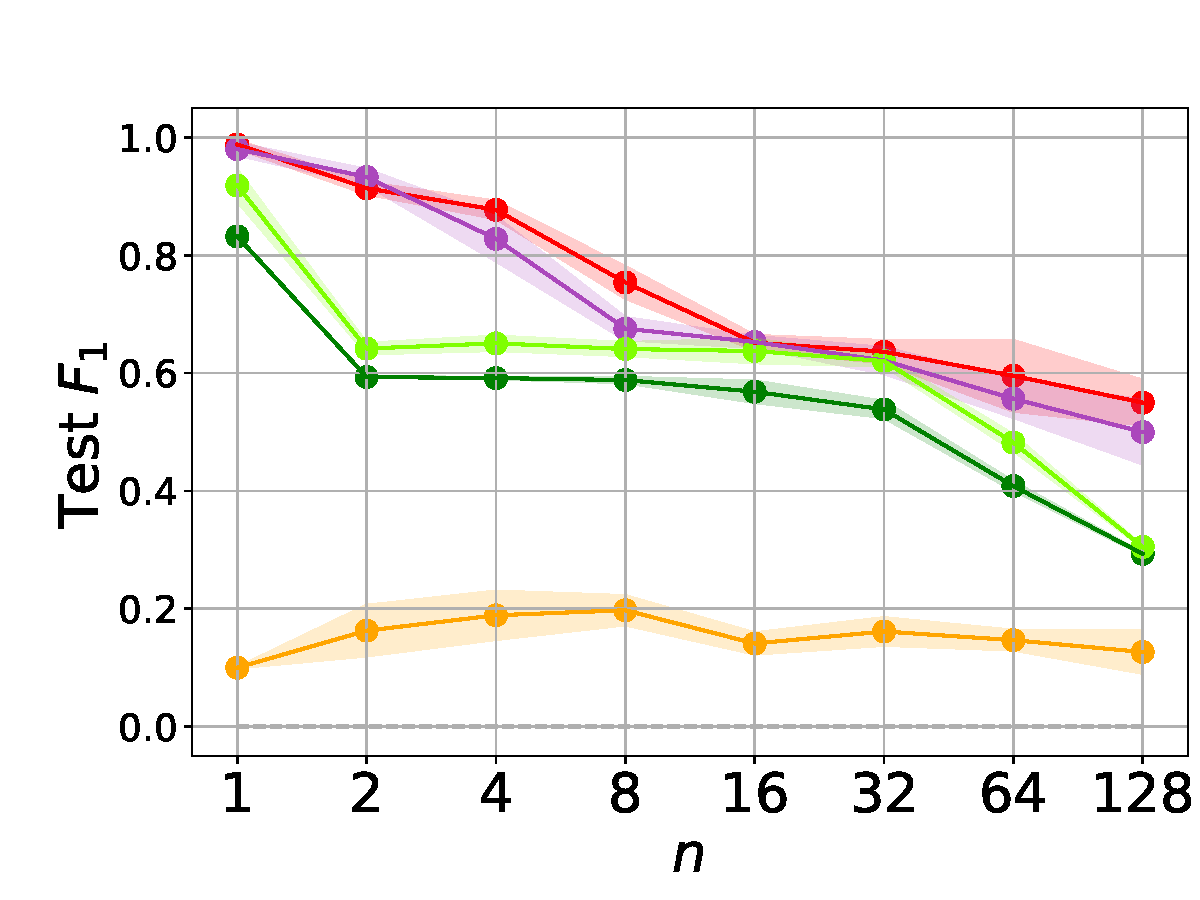
\includegraphics[width=\linewidth]{figs/periodicity/Fixed_ER/change_point/(2, n)DTDG_CP_Test $F_1$.pdf}
        \caption{DTDG - $\Pdet{2,n}$ - change.}
        \label{fig:dtdg_(2,n)_changepoints}
    \end{subfigure}
    \begin{subfigure}[b]{0.3\textwidth}
        \centering
        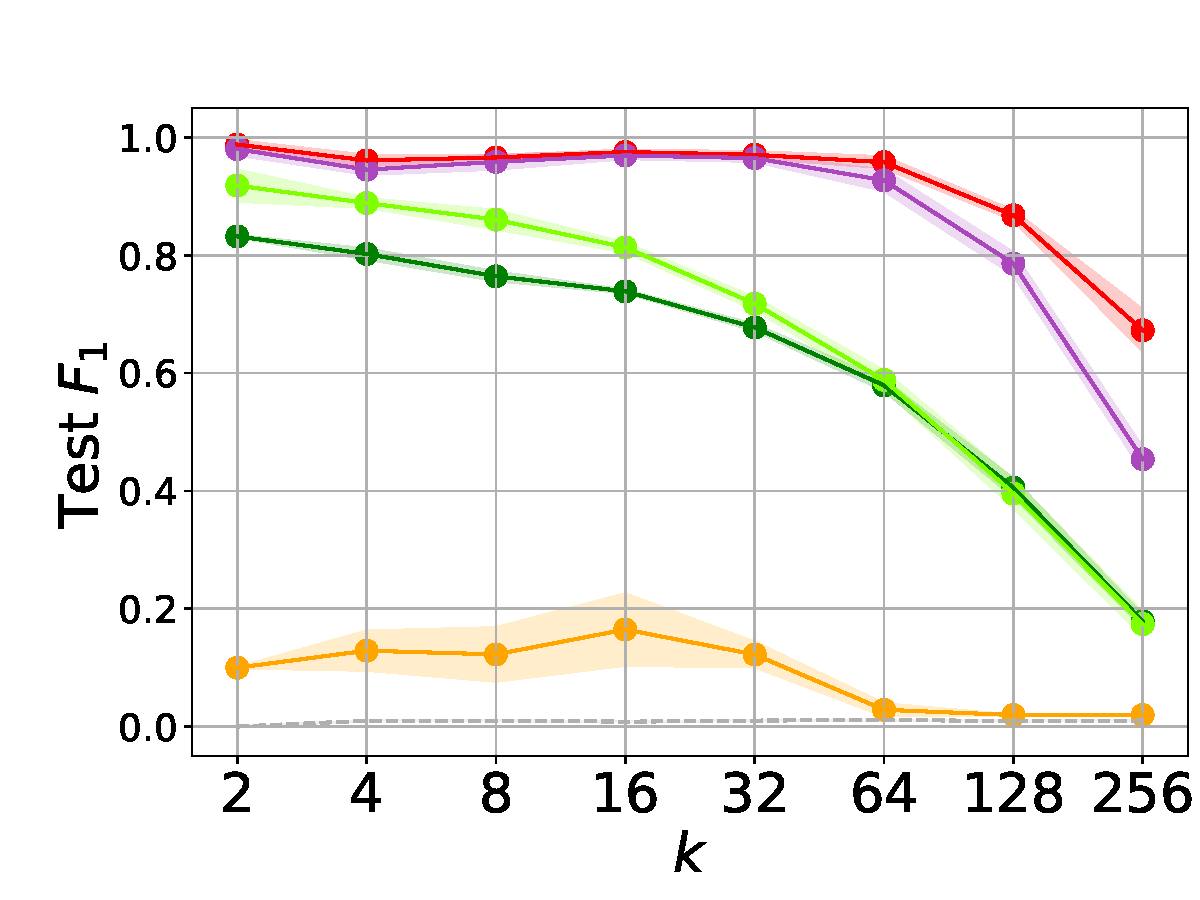
\includegraphics[width=\linewidth]{figs/periodicity/Fixed_ER/(k, 1)DTDG_Test $F_1$.pdf}
        \caption{DTDG - $\Pdet{k, 1}$ - All.}
        \label{fig:dtdg_(k, 1)}
    \end{subfigure}
    \begin{subfigure}[b]{0.08\textwidth}
        \centering
        \raisebox{14mm}{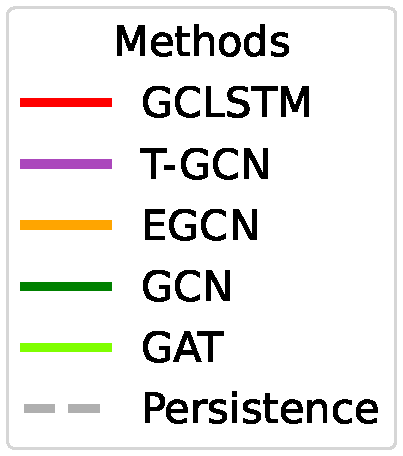
\includegraphics[width=\linewidth]{figs/legends/DTDG w persistence.pdf}}
    \end{subfigure}
    
    \caption{
    The six plots illustrate the performance of CTDG methods (top row) and DTDG methods (middle row) on the deterministic periodicity tasks $\Pdet{2, n}$ + $\Pdet{k, 1}$ (bottom row), alongside baseline methods (EdgeBank and Persistence), evaluated across both "All" and "Change point" timesteps. As $n$ increases, most CTDG and DTDG models maintain stable performance during the repetition phases but increasingly struggle to transition between the two graphs, ${G_1, G_2}$, at change points, exposing their limitations in accurate counting and switching. Furthermore, as $k$ increases, their memorization capacity deteriorates. Among the models, GCLSTM and DyGFormer consistently demonstrate strong and reliable performance on periodicity tasks overall.
    }
    \label{fig:det_periodic_overall}
\end{figure}

\paragraph{Multi-pattern periodicity $\Pdet{k, 1}$.}

In this setup, we further investigate the models' memorization capabilities by removing repetitiveness and introducing more diverse patterns within each period. As presented in Table~\ref{tab:det_periodic_datasets}, we generated eight multi-pattern datasets, where increasing $k$ results in a greater number of distinct snapshots, thereby making the memorization task more difficult.\\
Sub figures~\ref{fig:ctdg_(k, 1)} and ~\ref{fig:dtdg_(k, 1)} present the performance of CTDG, DTDG, and the baseline models on the $\Pdet{k, 1}$ datasets for different values of $k = \{2, 4, 8, 16, 32, 64, 128, 256\}$. All methods tend to gradually lose the memorization capacities for higher $k$. GCLSTM and DyGFormer consistently achieve the highest performance, even as $k$ increases, requiring the models to memorize a larger set of distinct patterns. TGCN, TGN, and TGAT perform robustly for $k <= 128$, while for $k=256$ there is a significant decrease in performance, . CTAN, EvolveGCN-O, and EvolveGCN-H underperform compared to static graph methods such as GCN and GAT, which do not utilize any temporal information. Edgebank gradually deteriorates in performance to even reaching zero for $\Pdet{256, 1}$, eventually defaulting to predicting each snapshot as a clique for larger $k$. \\
Given the weak performance of both EvolveGCN variants in both $\Pdet{2, n}$ and $\Pdet{k, 1}$ tasks, we report results only for EvolveGCN-O in the stochastic setting.


\subsubsection{Stochastic periodicity}

\begin{figure}[H]
    % (k, 1) CTDG
    \centering
    \begin{subfigure}[b]{0.44\textwidth}
        \centering
        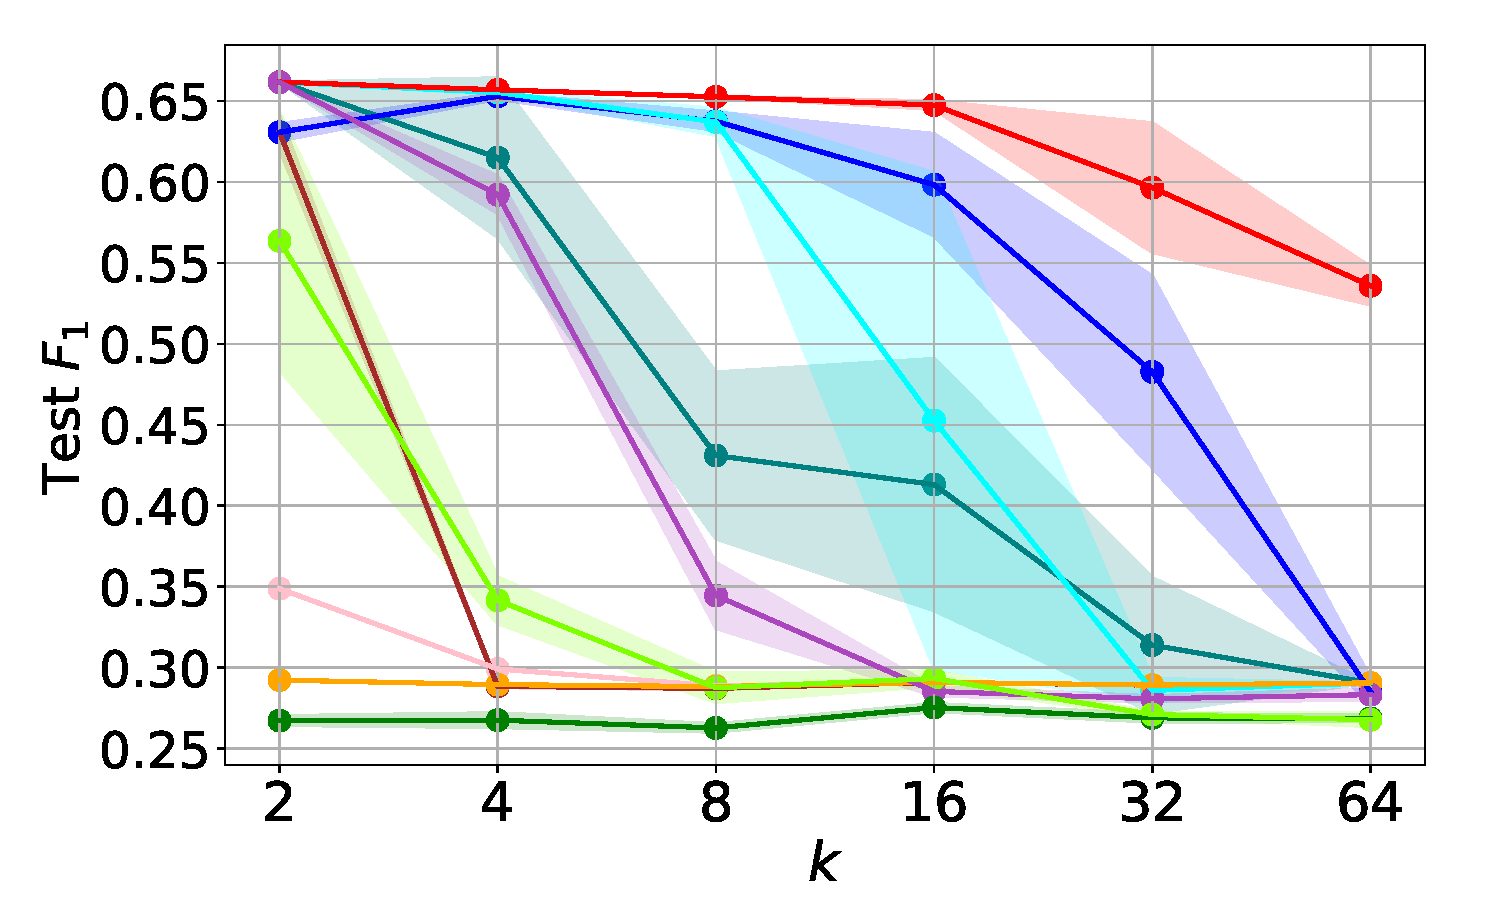
\includegraphics[width=\linewidth]{figs/periodicity/sbm_sto/V2/(0.5, 0.01)(k, 1)All_test avg_f1.pdf}
        \caption{All methods - $\mathcal{P}^{(\text{SBM})}(0.5)$}
        \label{fig:sub_all_(k, 1)_(0.5, 0.01)_sbm_sto}
    \end{subfigure}
    \hfill
    \begin{subfigure}[b]{0.44\textwidth}
        \centering
        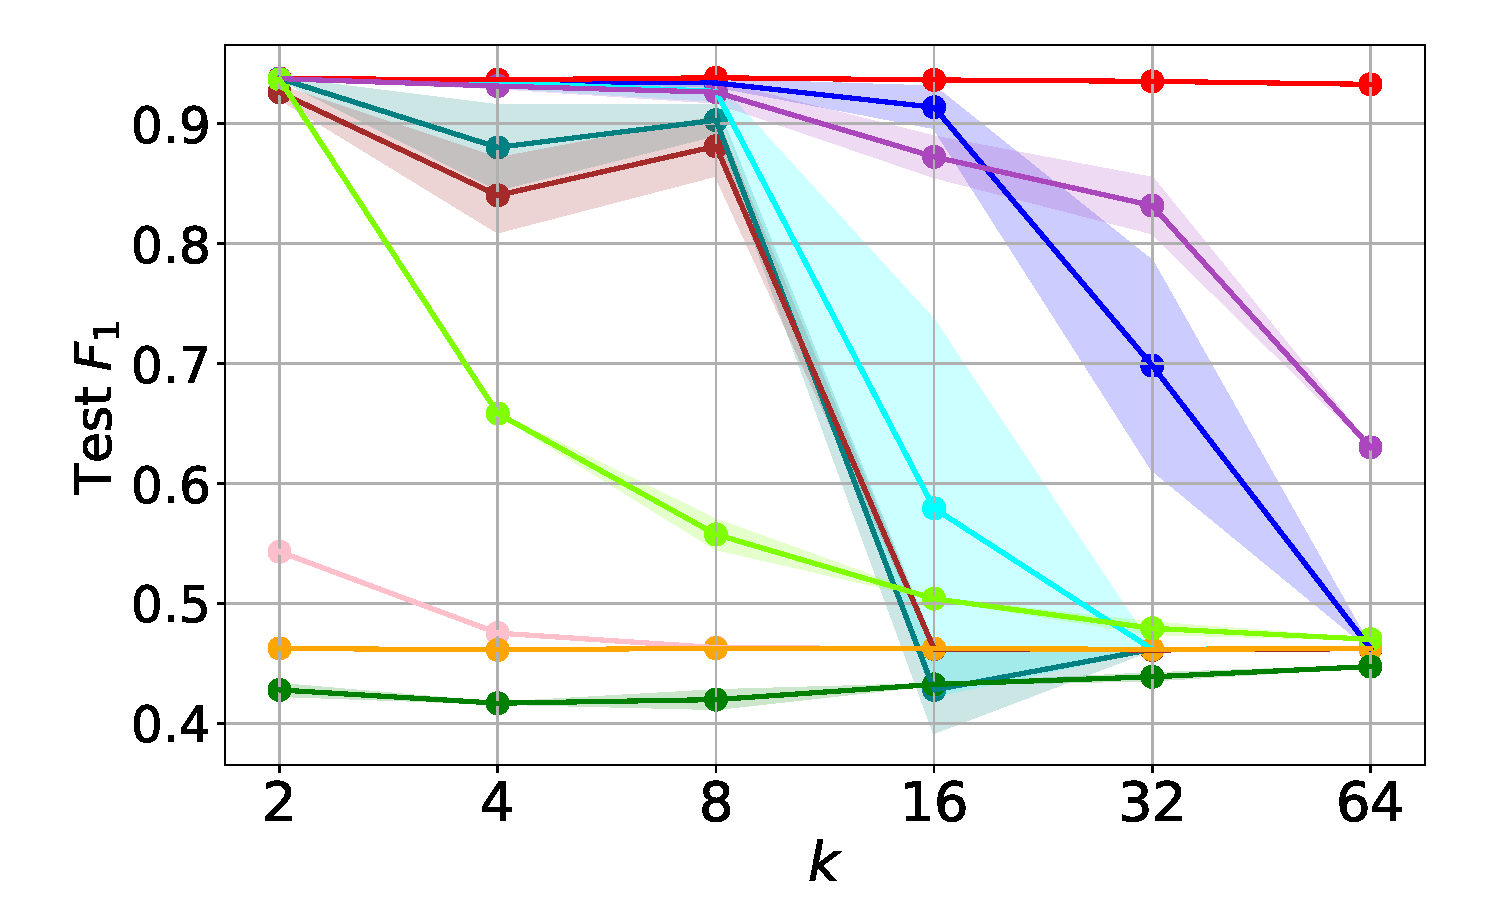
\includegraphics[width=\linewidth]{figs/periodicity/sbm_sto/V2/(0.9, 0.01)(k, 1)All_test avg_f1.pdf}
        \caption{All methods - $\mathcal{P}^{(\text{SBM})}(0.9)$}
        \label{fig:sub_all_(k, 1)_(0.9, 0.01)_sbm_sto}
    \end{subfigure}
    \begin{subfigure}[b]{0.1\textwidth}
        \centering
        \raisebox{15mm}{
        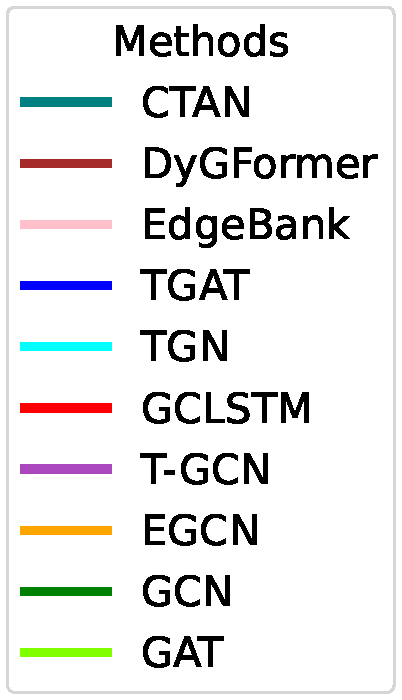
\includegraphics[width=\linewidth]{figs/legends/CTDG DTDG all w edgebank wo persistence.pdf}}
    \end{subfigure}
    
    \caption{}
    \label{fig:(K,1)_overall_sto}
\end{figure}


%if you need to divide in different parts, use \paragraphs

\subsubsection{Effect of number of neighbors}
To the best of our knowledge, the number of historical neighboring samples has not been systematically studied in temporal graph learning. In this work, we thoroughly investigate its effect on model training. Although increasing this value can provide richer historical context, it also introduces trade-offs in terms of greater computational overhead and extended training times.\\
Figure~\ref{fig:(K,1)_num_neighbors_det} presents the performance of CTDG methods on $\Pdet{k, 1}$ across different numbers of neighboring samples for K=32, 64, and 256. DyGFormer demonstrate strong generalization across varying historical sampling sizes, whereas CTAN and TGN are highly sensitive, with both showing substantial improvement when provided with the same period length for $\Pdet{64, 1}$ and $\Pdet{256, 1}$. 
TGAT represents the low-sensitivity for smaller $k$ values, i.e. $k = \{32, 64\}$, while substantially getting a decent performance when the number of neighbors is twice as period length. \\
As illustrated in Figure~\ref{fig:(K,1)_num_neighbors_sto}, we examined the effect of the number of neighboring samples in a stochastic setting using Stochastic Block Model (SBM) to sample the graph sequences $\mathcal{G}$, with intra- and inter-cluster probabilities of 0.9 and 0.01. our reinforces our observations from the deterministic setting: increasing the number of neighboring samples tends to facilitate more effective training. However, certain exceptions exist. For example, TGN on $\Psto{16, 1}$ with 128 neighboring samples exhibited training instability.


\begin{observation}[Effect of Number of Neighbors]
The number of temporal neighbors sampled significantly affect model performance for CTDG methods. 
\end{observation}

\begin{figure}[H]
    % (k, 1) CTDG
    \centering
    \begin{subfigure}[b]{0.44\textwidth}
        \centering
        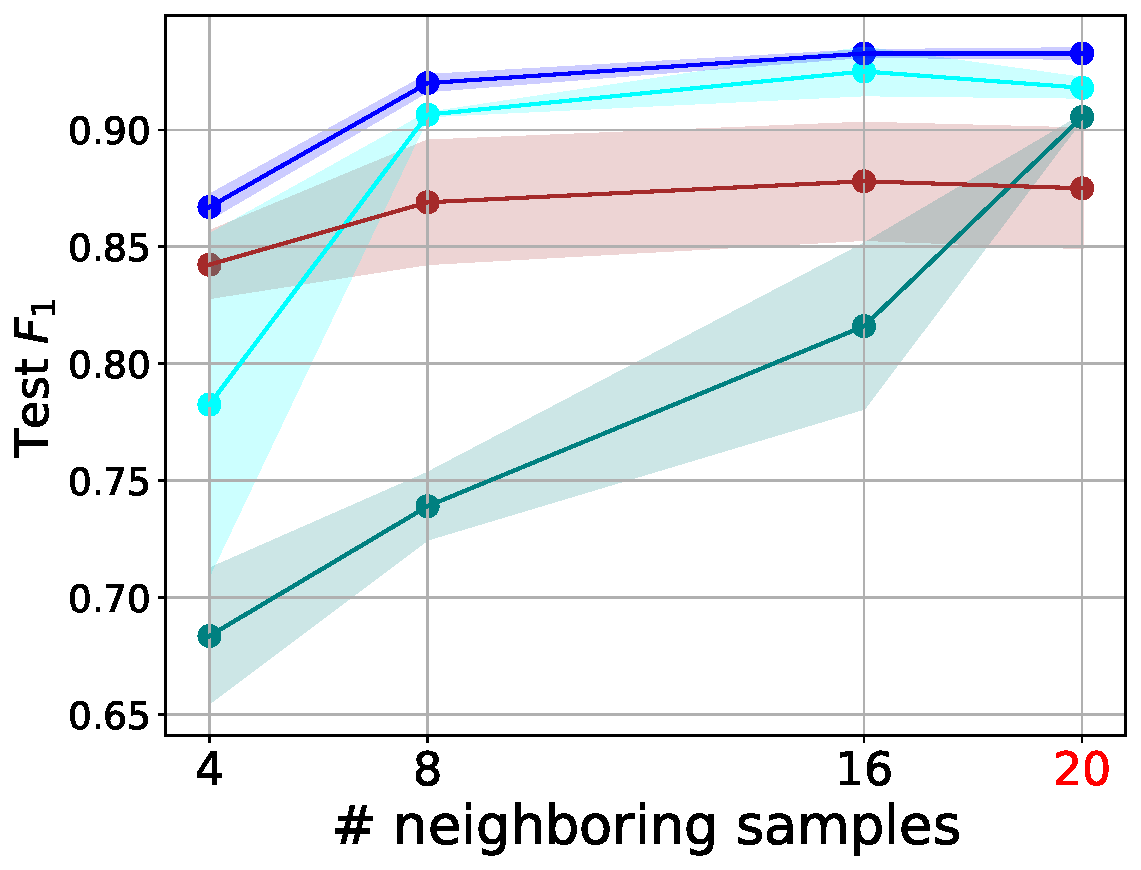
\includegraphics[width=\linewidth]{figs/periodicity/sbm_sto/V2/num_neighboring/multi_seed/(8,1)(0.9, 0.01).pdf}
        \caption{$\Psto{8, 1}$}
        \label{fig:sub_all_(k, 1)_(0.5, 0.01)_sbm_sto}
    \end{subfigure}
    \hfill
    \begin{subfigure}[b]{0.44\textwidth}
        \centering
        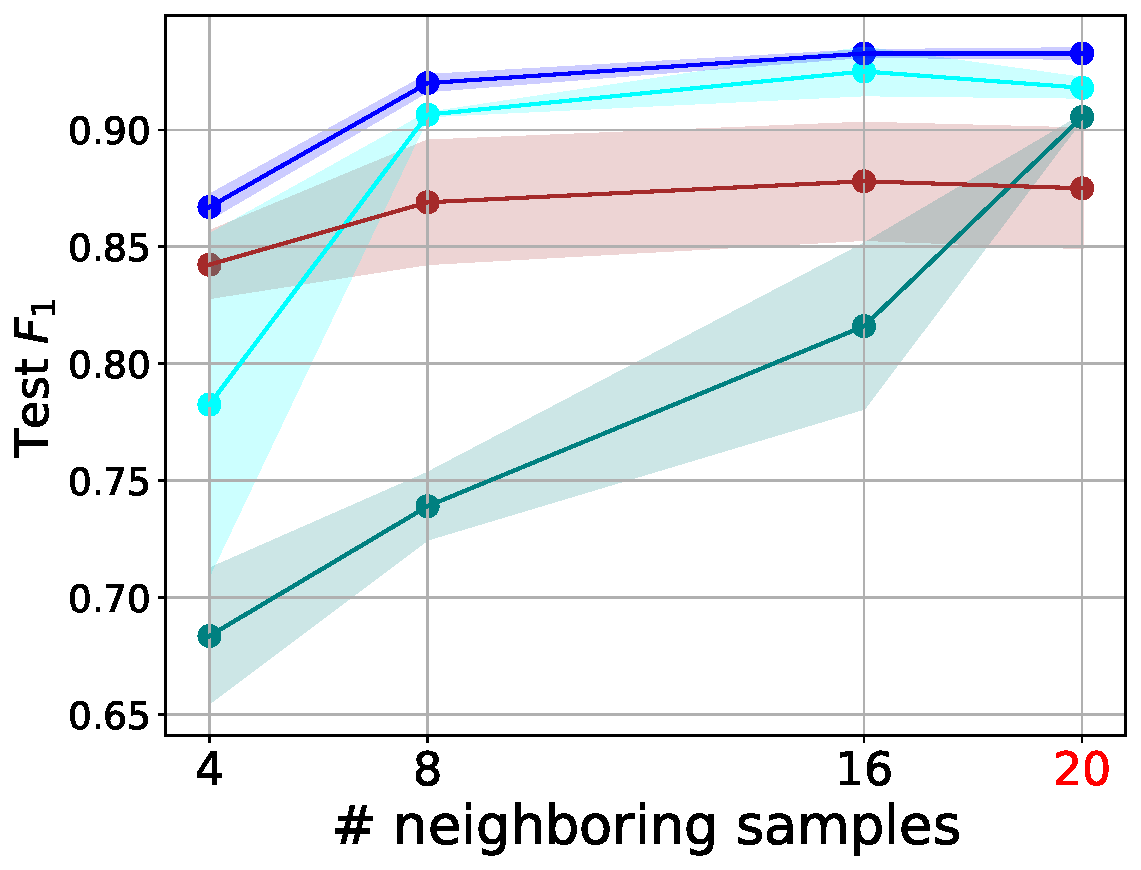
\includegraphics[width=\linewidth]{figs/periodicity/sbm_sto/V2/num_neighboring/multi_seed/(8,1)(0.9, 0.01).pdf}
        \caption{$\Pdet{256, 1}$}
        \label{fig:sub_all_(k, 1)_(0.9, 0.01)_sbm_sto}
    \end{subfigure}
    
    \caption{}
    \label{fig:periodicity_multi_seed_neighbors}
\end{figure}

% For further investigation, This motivates us to train TGN with three different number of neighbors, as depicted at Figure~\ref{fig:(K,1)_TGN}: the default 20 ("TGN"), a size equal to the period length ("TGN-K"), and double the period length ("TGN-2K"). Empirically, TGN performs significantly better when using twice the period length, surpassing both the default 20 and the same-size period settings. \\

\begin{figure}[H]
    % (k, 1) CTDG
    \centering
    \begin{subfigure}[b]{0.24\textwidth}
        \centering
        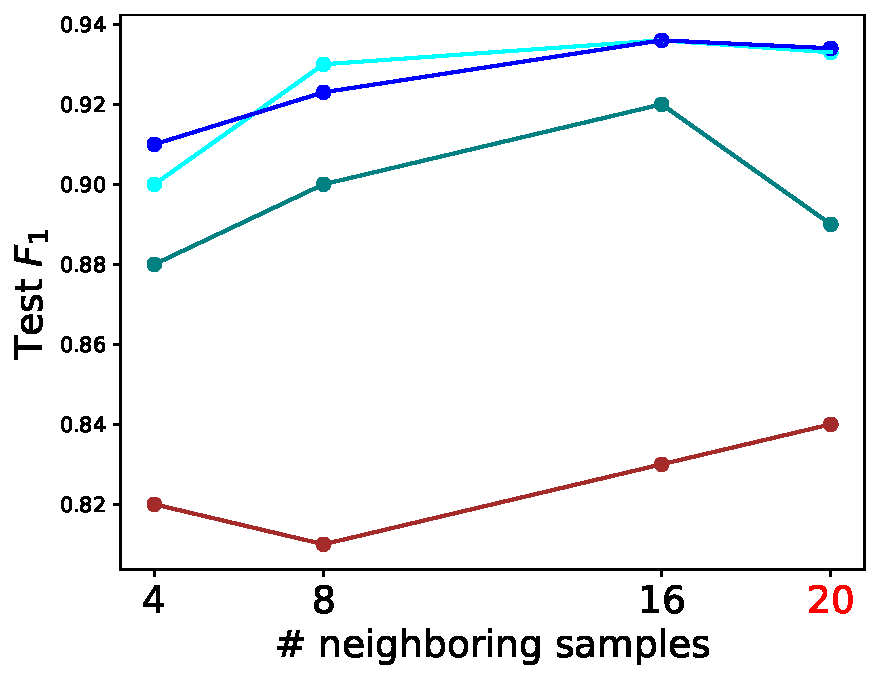
\includegraphics[width=\linewidth]{figs/periodicity/sbm_sto/V2/num_neighboring/(4, 1)(0.9, 0.01).pdf}
        \caption{$\Psto{4, 1}$}
        \label{fig:sub_num_neighbors_sto_(4,1)}
    \end{subfigure}
    \begin{subfigure}[b]{0.24\textwidth}
        \centering
        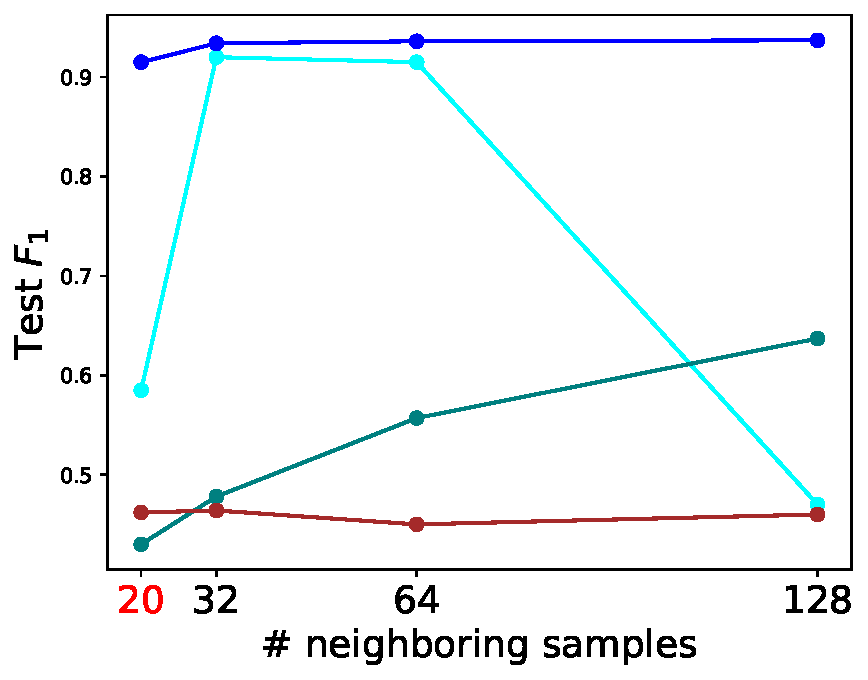
\includegraphics[width=\linewidth]{figs/periodicity/sbm_sto/V2/num_neighboring/(16, 1)(0.9, 0.01).pdf}
        \caption{$\Psto{16, 1}$}
        \label{fig:sub_num_neighbors_sto_(16,1)}
    \end{subfigure}
    \begin{subfigure}[b]{0.24\textwidth}
        \centering
        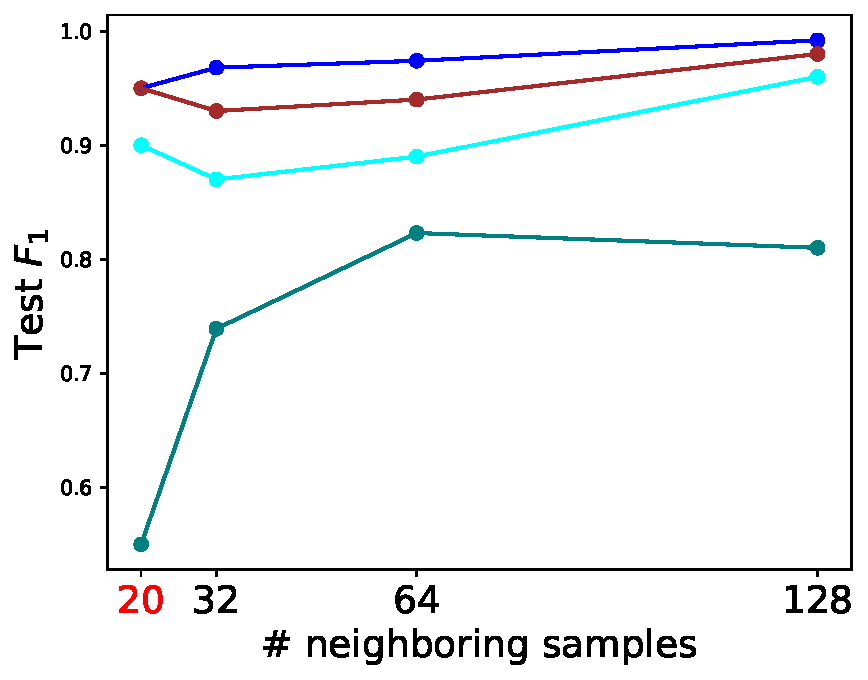
\includegraphics[width=\linewidth]{figs/periodicity/Fixed_ER/num_neighboring/(32,1).pdf}
        \caption{$\Pdet{32, 1}$}
        \label{fig:sub_num_neighbors_det_(32,1)}
    \end{subfigure}
    \begin{subfigure}[b]{0.24\textwidth}
        \centering
        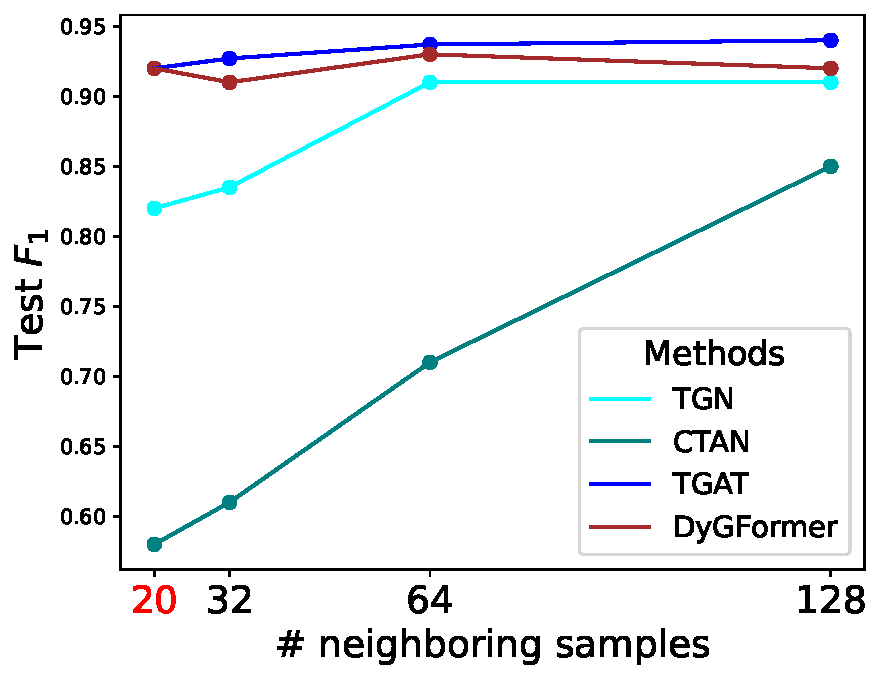
\includegraphics[width=\linewidth]{figs/periodicity/Fixed_ER/num_neighboring/(64,1).pdf}
        \caption{$\Pdet{64, 1}$}
        \label{fig:sub_num_neighbors_det_(64,1)}
    \end{subfigure}
    \caption{We evaluate the effect of the number of historical neighboring samples in CTDG methods across three multi-pattern deterministic periodic tasks: $\Pdet{32, 1}$, $\Pdet{64, 1}$, and $\Pdet{256, 1}$. The red-highlighted value denotes the default number of neighboring samples used in most experiments. The results show that CTAN and TGN are highly sensitive to this parameter, with their performance improving considerably as more neighboring samples are provided. In contrast, DyGFormer exhibits strong robustness and generalization, maintaining stable performance even when fewer neighboring samples are available. We investigate how the number of historical neighboring samples affects the performance of CTDG methods on three multi-pattern stochastic periodic tasks: $\Psto{4, 1}$, $\Psto{8, 1}$, and $\Psto{16, 1}$. The value highlighted in red represents the default setting used in most experiments. In general, increasing the number of neighboring samples improves performance. However, TGN encounters training instability on $\Psto{16, 1}$ when using 128 neighboring samples, highlighting the importance of carefully tuning this hyperparameter.}
    \label{fig:(K,1)_num_neighbors_det}
\end{figure}


\subsection{Delayed Cause and Effect Task}

\begin{figure}[H]
    % (k, 1) CTDG
    \centering
    \begin{subfigure}[b]{0.29\textwidth}
    \centering
    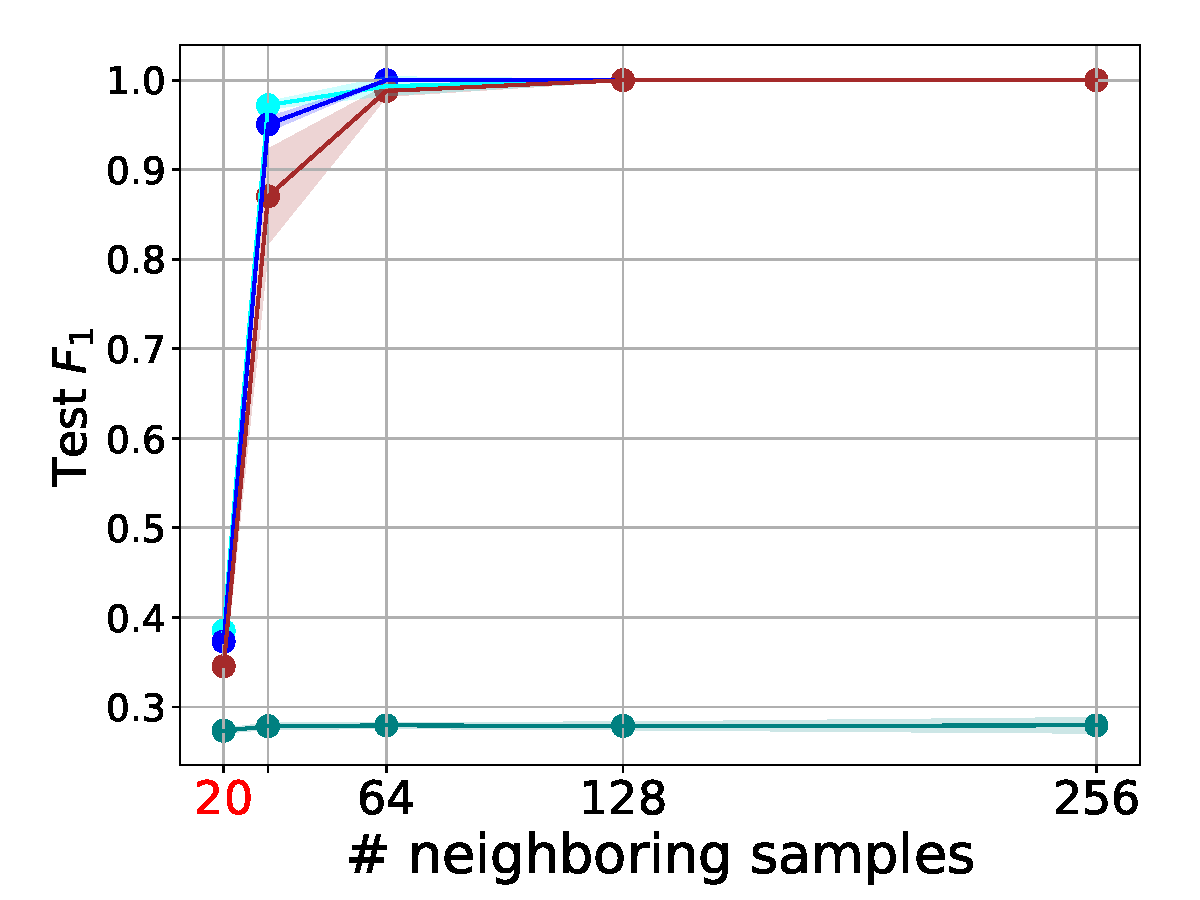
\includegraphics[width=\linewidth]{figs/memory_node/num_neighbors/(64,4000).pdf}
    \caption{CTDG methods - $\ell=64$}
    \end{subfigure}
    \begin{subfigure}[b]{0.29\textwidth}
    \centering
    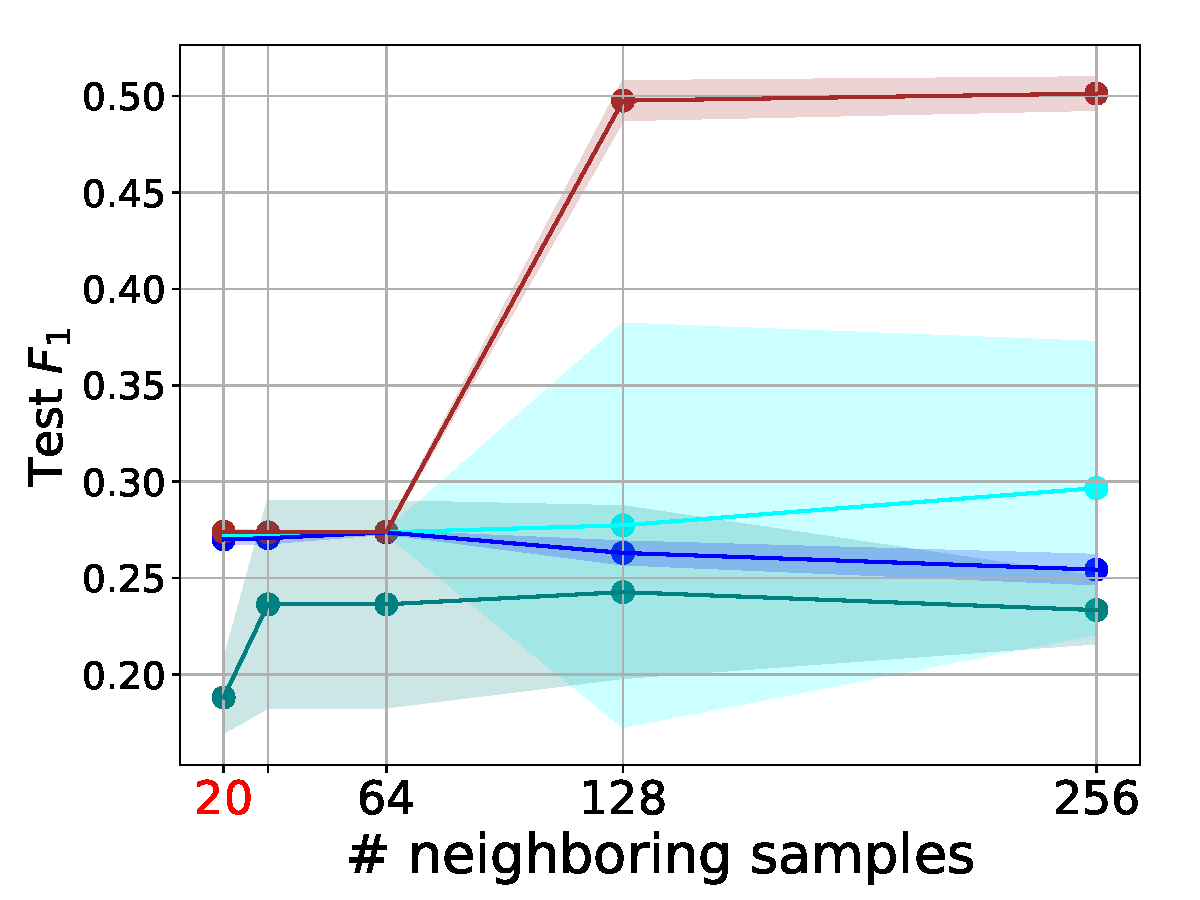
\includegraphics[width=\linewidth]{figs/memory_node/num_neighbors/(256,4000).pdf}
    \caption{CTDG methods - $\ell=256$}
    \end{subfigure}
    \begin{subfigure}[b]{0.29\textwidth}
    \centering
    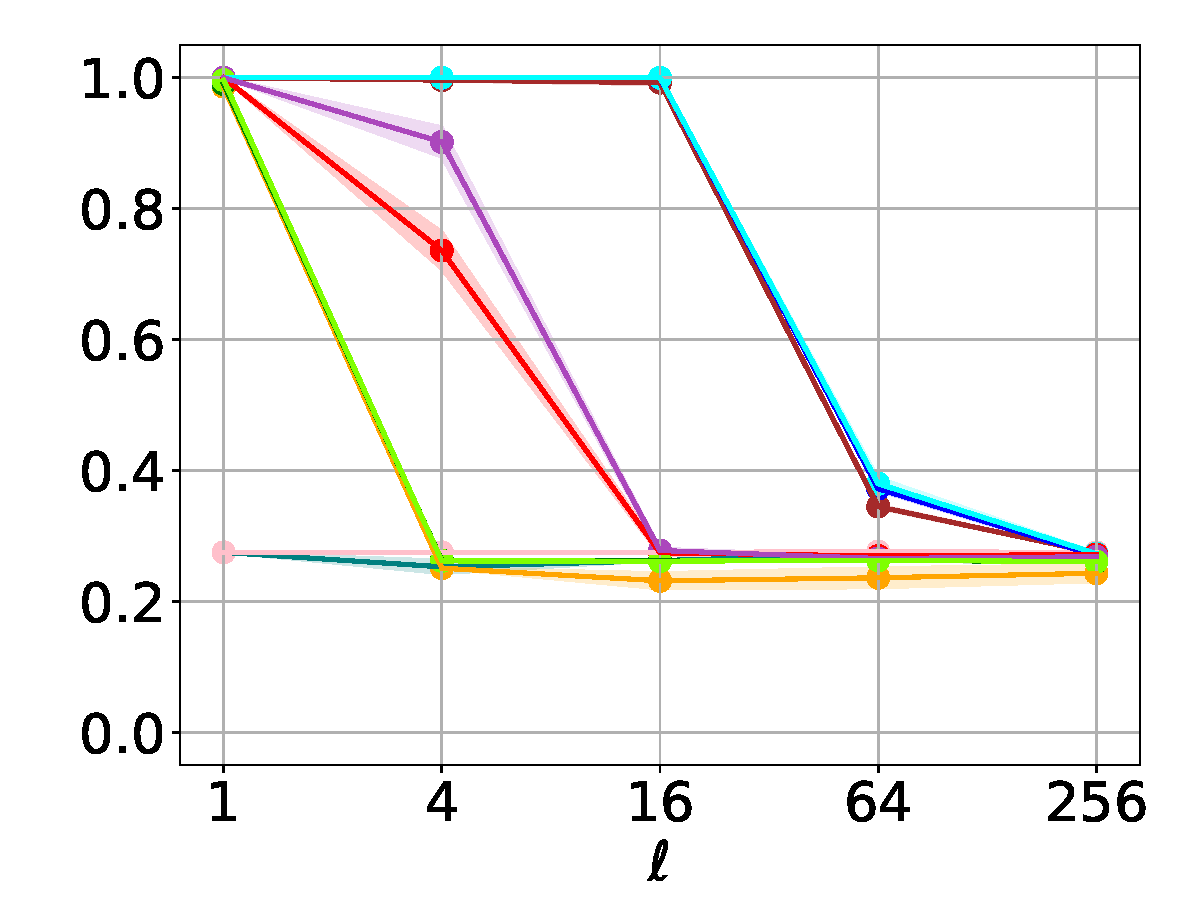
\includegraphics[width=\linewidth]{figs/memory_node/(8, 6)/(l)Best_Test $F_1$.pdf}
    \caption{All methods}
    \end{subfigure}
    \begin{subfigure}[b]{0.1\textwidth}
        \centering
        \raisebox{10mm}{
    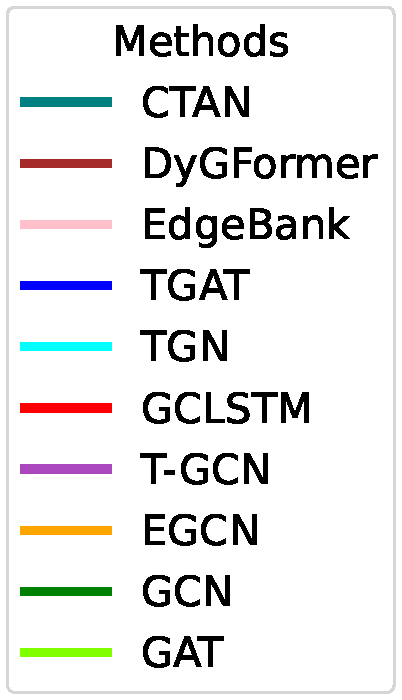
\includegraphics[width=\linewidth]{figs/legends/CTDG DTDG all w edgebank wo persistence.pdf}}
        \end{subfigure}
    \caption{}
    \label{fig:plot_mem_node}
\end{figure}

\subsubsection{Effect of number of neighbors}

\subsection{Spatial Long Range Dependencies Task}
% We fix $P=3$, and $n=12$, vary spatial distance $d \in \{1,2,4,8,16\}$ and temporal lag $l \in \{1,4, 16, 32\}$. For each $(l, d)$ we generate $2048$ timestep and split them $80/10/10\%$ (preserving entire lagged patterns), and report the average test $f_1$  score on the edge linking the target node $T$ to the endpoints of the $P$ path.
% In this section, we assess each of out selected method's ability to jointly reason over both spatial and temporal distances using the Long-Range Spatial-Temporal task (definition \ref{def:long_range}). 
In our experimental setup (Figure~\ref{fig:longrange}), we fix the number of paths at $P=3$ and use $n=100$ intermediary nodes, while varying the spatial distance $d \in \{1, 2, 4, 8, 16\}$ and the temporal lag $\ell \in \{1, 4, 16, 32\}$. Nodes indexed as $0$ and $1$ are designated as the source ($S$) and target ($T$) nodes, respectively.
 For each $(l, d)$ we generate $4000 + \ell$ timesteps, ensuring target $T$ has links at the last $4000$ timesteps. We split them $80/10/10\%$ (preserving entire lagged patterns), and report the average test $F_1$  score on the edge linking the target node $T$ to the endpoints of the $P$ path. All results are average over five random seeds. Figure \ref{fig:plots_long_range} plots $F_1$ vs. $d$ for lags $\ell=1,4,16,32$. \\
One can look at this figure as it shows how performance degrades as paths lengthen. When $\ell=1$ the four CTDG models (DyGFormer, TGAT, CTAN, TGN) stat near an $F_1 = 100\%$ and decline only modestly to near $F_1 = 95\%$.
% except TGAT, t
This shows that most of these methods can capture spatial dependencies without considering the temporal lag as they have near perfect performance in $\ell=1$.
% near-instant temporal effect, which eliminate the need for any temporal understanding for these tasks and as it was expected all methods except TGAT, which is specifically is designed to capture temporal dependencies, have near perfect performance. 
As we increase lag to $\ell=4$, the first thing to notice is the decline for both DTDG methods (GCLSTM and T-GCN).
% where GCLSTM is only able to capture one hub information with increased lag and both DTDG methods fail to capture any more than that $2$ hub information in a long-delay effects ($\ell=4$), 
Whereas CTDG methods perform descent up until $D=4$ and after that they decline as well and it's only DyGFromer which its $F_1$ remain higher that $80\%$ for larger distances. \\
Moving on to $\ell=16$, as expected DTDG method are completely failing to learn any information for this taks but CTDG methods still perform descent. 
TGN and TGAT hold higher $F_1$ and surpassing DyGFormer.
% Only thing that catch eyes in this experiment is the good performance of TGN and TGAT and the fact that they perform better that DyGFormer is unexpected since DyGFormer outperforms both these methods for almost all the previous experiments. Another surprising result from this plot can be observed from performance of TGAT and TGN for distance $d = 4, 8$, where going up from $4$ to $8$ doesn't seem to have changed the average performance of these methods.
For the longest delay $\ell=32$, the general trend stay consistent with previous plots and every methods collapse to $F_1=0$ at $d=16$. \\
CTDG methods vastly outperform DTDG ones but still degrade for extreme $(l, d)$. TGAT and TGN maintain perfect accuracy for $d \leq 2$ across all lags, which highlights their strength on short-range patterns independent of time and we think is because of their specialized temporal designs. \\ 
These results also confirm that no model can handle the most extreme spatial-temporal dependencies, limited capacity and insufficient temporal leverage prevent them from storing and retriving information across long delays and distances (e.g., TGAT would need an impractically large $2^{(\textit{Nodes} \times \ell \times d)}$ attention matrix to solve this task). 
The performance plateau of TGAT and TGN and $d=4$ to $d=8$ for delay $\ell=16$, indicates they exhaust their temporal storage before their spatial encoding limits.

% Relying on these observation we claim that none of these methods can learn to extract necessary information to solve this task, this can be because of the general low capacity of the models and the model's failure to capture complexity of these task as they have not enough temporal leverage in their architectures, for empale TGAT, needs to store all $16$ hubs neighbor information for at least $32$ time-steps before, to be able to correctly solve this task and this only requires an attention matrix of approximate size $2^{18}$, for each occurring pattern which is way out of TGAT capacity. It's noteworthy to mention that TGAT and TGN performance on distances $d=4, 8$ stay the same only for $\ell=16$ which raise another ambiguity for explaining these results. This can only happen in a senario where TGAT and TGN learn some delays for all 16 steps (we estimate they learn $80\%$ of these every $16$ repeating patterns, which is about $13$ patterns)
% Our hypothesis is that these two methods reach their full temporal capacity when capturing $d=4, l=16$ but not their full spatial capacity as they still can learn the same amount of patterns (around $13$) for distance $d=8$. Moreover, TGAT and TGN have near perfect performance with very low variance for distance $1, 2$, for both all lags $\ell = 1,4, 16,32$ which suggests that these two methods can capture any structural dependencies up to $2$-hub neighbor information for the mentioned lags, which in itself shows the ability of these -temporally-specific crafted methods to capture long-range dependencies in comparison to other methods.
% All in all, our experiments in this section verify that despite the fact that some methods can capture long-appearing patterns in datasets most GNN methods fail to capture delayed patterns, spatially separated dependencies.



\begin{figure}[H]
    % (k, 1) CTDG
    \centering
    \begin{subfigure}[b]{0.24\textwidth}
        \centering
        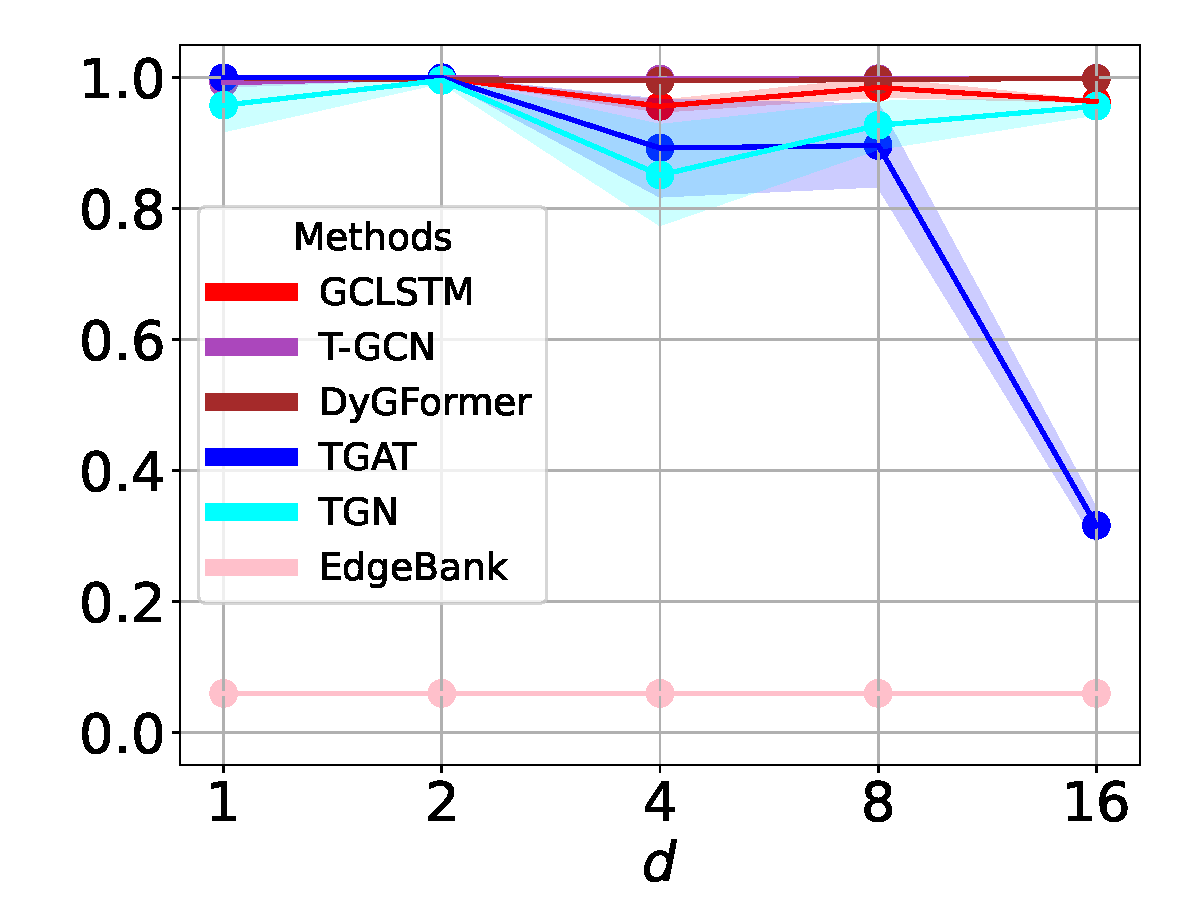
\includegraphics[width=\linewidth]{figs/long_range/fig(10, 10)/(1, d)Best_Test $F_1$.pdf}
        \caption{$(\ell=1, d)$}
        \label{fig:sub_long_range_(1,d)}
    \end{subfigure}
    \begin{subfigure}[b]{0.24\textwidth}
        \centering
        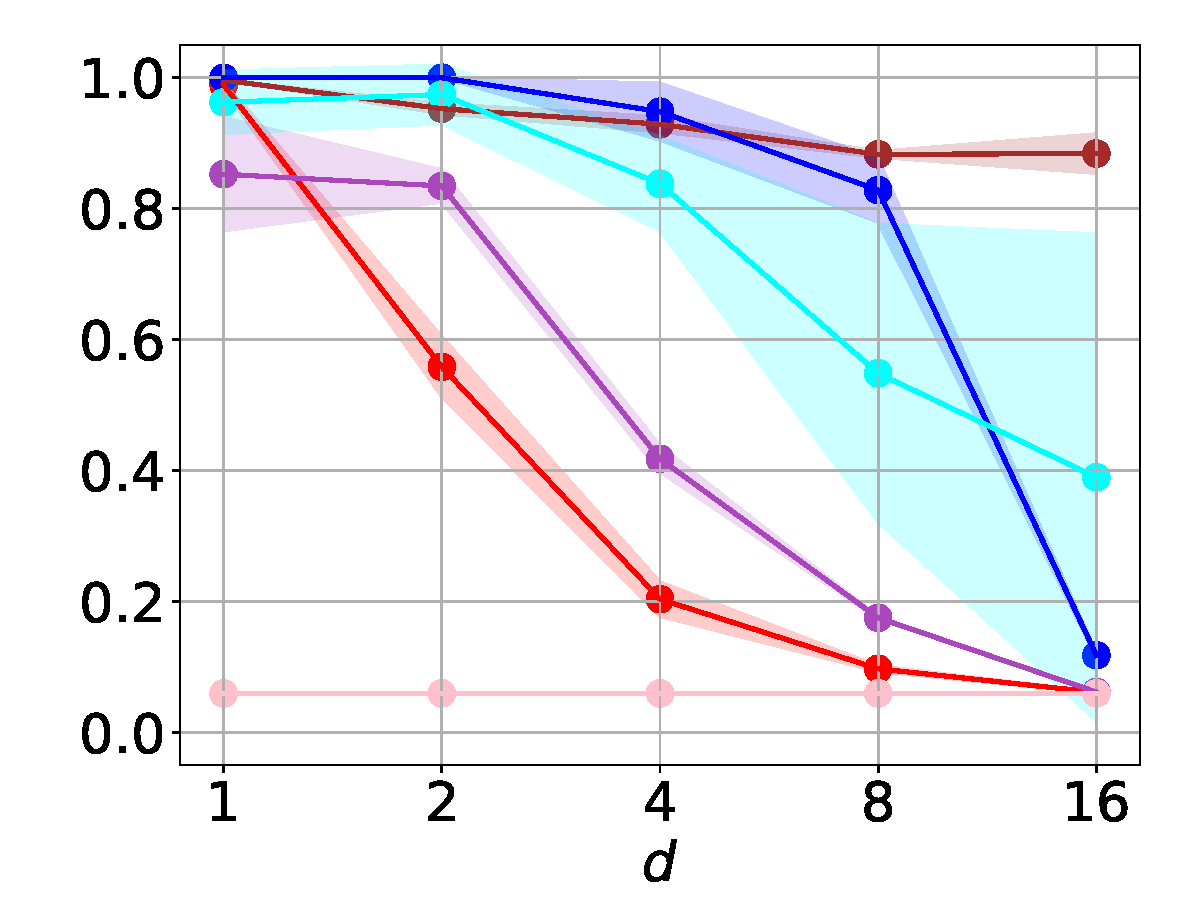
\includegraphics[width=\linewidth]{figs/long_range/fig(10, 10)/(4, d)Best_Test $F_1$.pdf}
        \caption{$(\ell=4, d)$}
        \label{fig:sub_long_range_(4,d)}
    \end{subfigure}
    %(k, 1) DTDG
    \centering
    \begin{subfigure}[b]{0.24\textwidth}
        \centering
        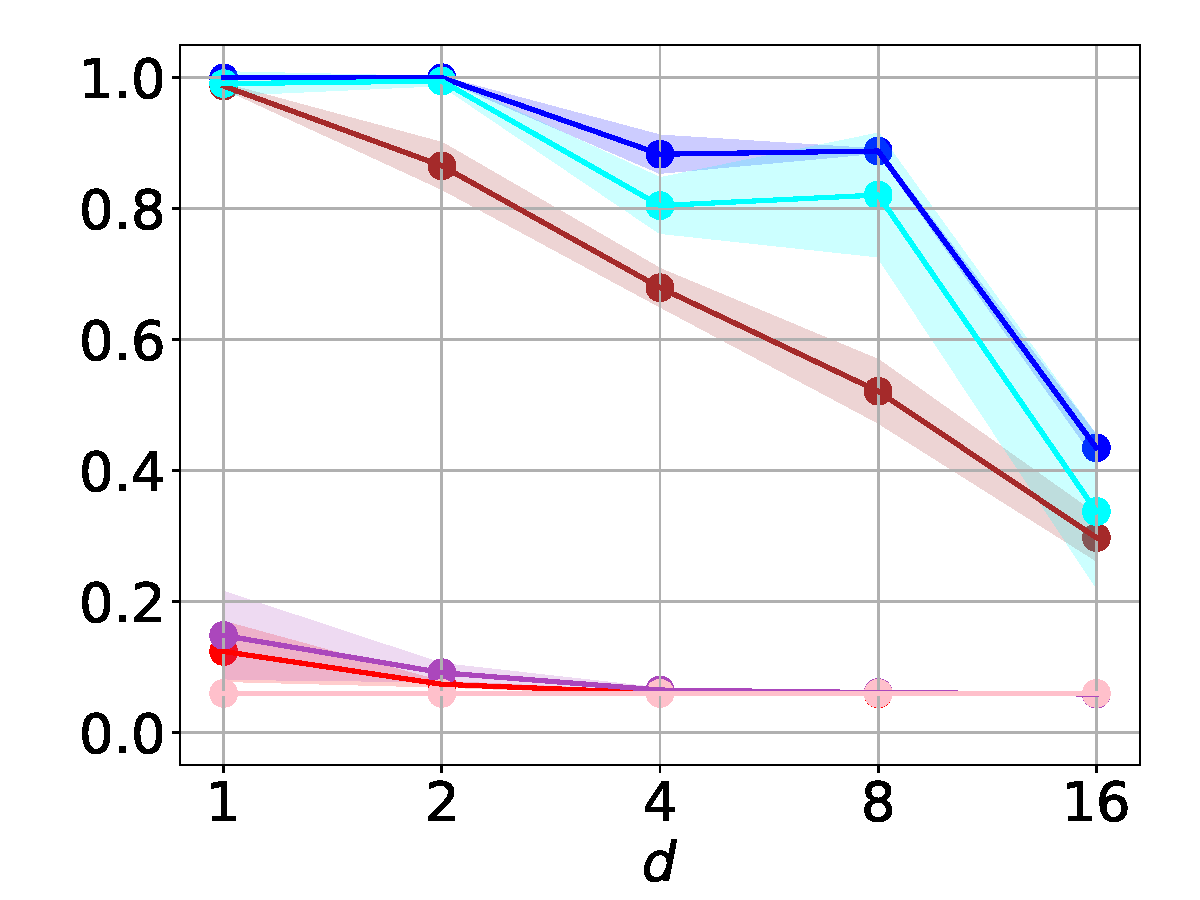
\includegraphics[width=\linewidth]{figs/long_range/fig(10, 10)/(16, d)Best_Test $F_1$.pdf}
        \caption{$(\ell=16, d)$}
        \label{fig:sub_long_range_(16,d)}
    \end{subfigure}
    \begin{subfigure}[b]{0.24\textwidth}
        \centering
        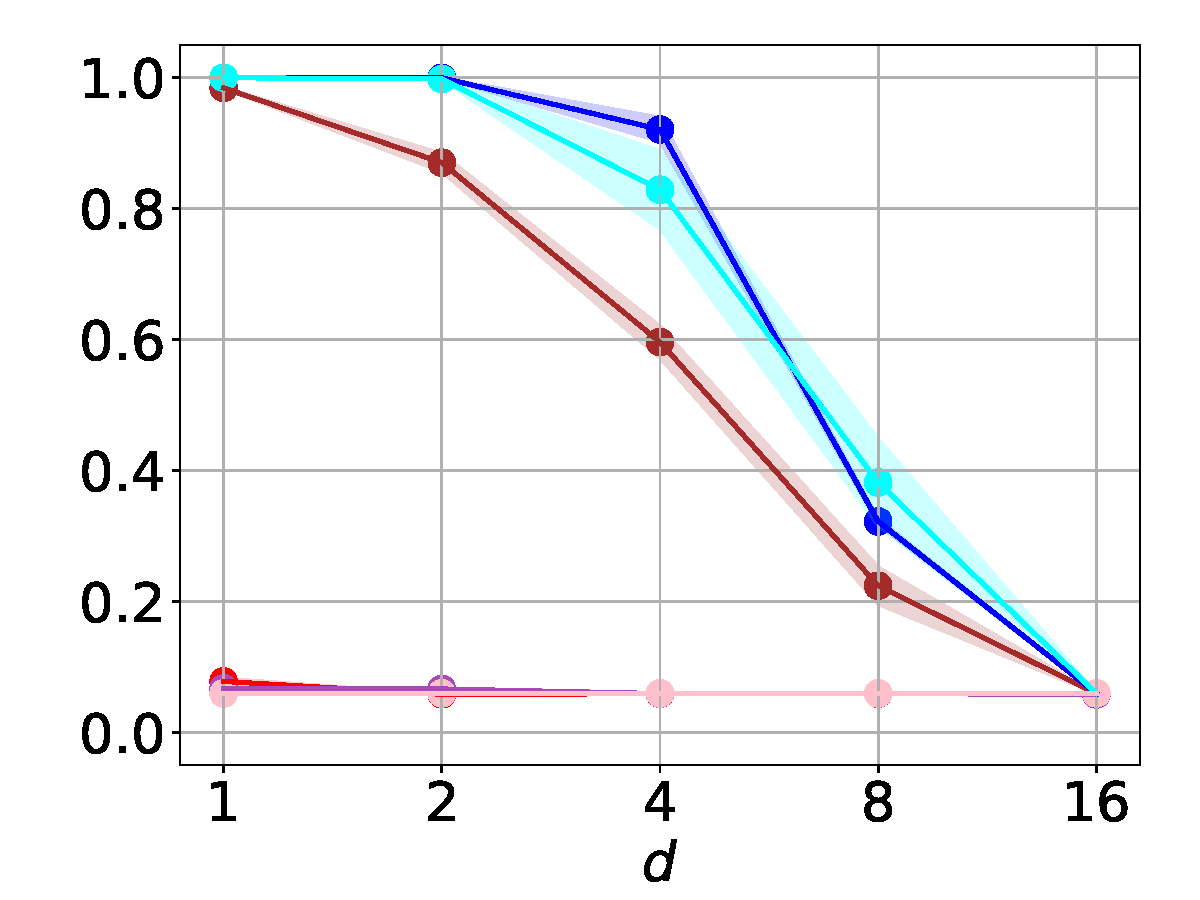
\includegraphics[width=\linewidth]{figs/long_range/fig(10, 10)/(32, d)Best_Test $F_1$.pdf}
        \caption{$(\ell=32, d)$}
        \label{fig:sub_long_range_(32,d)}
    \end{subfigure}
    
    \caption{We evaluate the performance of GCLSTM, TGCN, TGAT, TGN, DyGFormer, and EdgeBank on spatial long-range dependency tasks with varying temporal dependencies $(\ell = \{1, 4, 16, 32\}, d)$. As the temporal dependency length $\ell$ increases, DTDG models experience a sharp decline in performance, whereas CTDG models show greater robustness. When $\ell=1$ (very short temporal dependency), all models maintain stable performance with respect to spatial dependency. However, as both $\ell$ and spatial dependency increase, performance consistently degrades. At higher $\ell$ values, DyGFormer progressively loses spatial understanding, while TGCN and GCLSTM approach an $F_1$ score near zero, indicating a failure to capture spatial dependencies reliably. Among the models, TGAT and TGN remain comparatively more resilient, though they too gradually lose spatial awareness as temporal dependencies grow.}
    \label{fig:plots_long_range}
\end{figure}




% \end{document}